\documentclass[oneside]{book}

\usepackage{amssymb}
\usepackage{graphicx}
\usepackage{eufrak}

\newtheorem{theorem}{Theorem}[chapter]
\newtheorem{lemma}[theorem]{Lemma}
\newtheorem{proposition}[theorem]{Proposition}
\newtheorem{corollary}[theorem]{Corollary}

\newenvironment{proof}[1][Proof]{\begin{trivlist}
\item[\hskip \labelsep {\bfseries #1}]}{\end{trivlist}}
\newenvironment{definition}[1][Definition]{\begin{trivlist}
\item[\hskip \labelsep {\bfseries #1}]}{\end{trivlist}}
\newenvironment{example}[1][Example]{\begin{trivlist}
\item[\hskip \labelsep {\bfseries #1}]}{\end{trivlist}}
\newenvironment{remark}[1][Remark]{\begin{trivlist}
\item[\hskip \labelsep {\bfseries #1}]}{\end{trivlist}}

\newcommand{\qed}{\nobreak \ifvmode \relax \else
      \ifdim\lastskip<1.5em \hskip-\lastskip
      \hskip1.5em plus0em minus0.5em \fi \nobreak
      \vrule height0.75em width0.5em depth0.25em\fi}

\begin{document}
\title{Notes and Solutions for ``Measure Theory and Integration" by Michael E. Taylor}
\author{Arya Pourzanjani} 
\date{\today}
\maketitle

%%%%%%%%%%%%%%%%
%%%%%%%%%%%%%%%%
\chapter{The Riemann Integral}
%%%%%%%%%%%%%%%%
%%%%%%%%%%%%%%%%

\section*{Solutions}
\begin{enumerate}
%%%%%%%%%
%%%%%%%%%
\item[7.] Since $f:[ac,bc]\to \mathbb{R}$ is Riemann integrable, by definition its integral is equal to its upper sum i.e.

\begin{eqnarray}
\label{eq:upperSumStretched}
\frac{1}{c}\int_{ac}^{bc} f(x)\,dx &=& \frac{1}{c} \inf_{\cal{P}} \bar{I}_{\cal{P}}(f) \nonumber \\
&=& \frac{1}{c} \inf_{\cal{P}} \sum_{k} \sup_{[x_k,x_{k+1}]} f(x)\, l([x_k,x_{k+1}])
\end{eqnarray}

Assume $c > 1$ for the sake of intuition here. They key insight to note here is that by multiplying the input of a function by a constant i.e. $f(cx)$ we effectively make it so that when going from left to right the function ``reaches" the numbers in its range earlier than it normally would and the function appears shrunken. Figure \ref{fig:sinSpedUp} shows an example.

\begin{figure}[h]
    \centering
    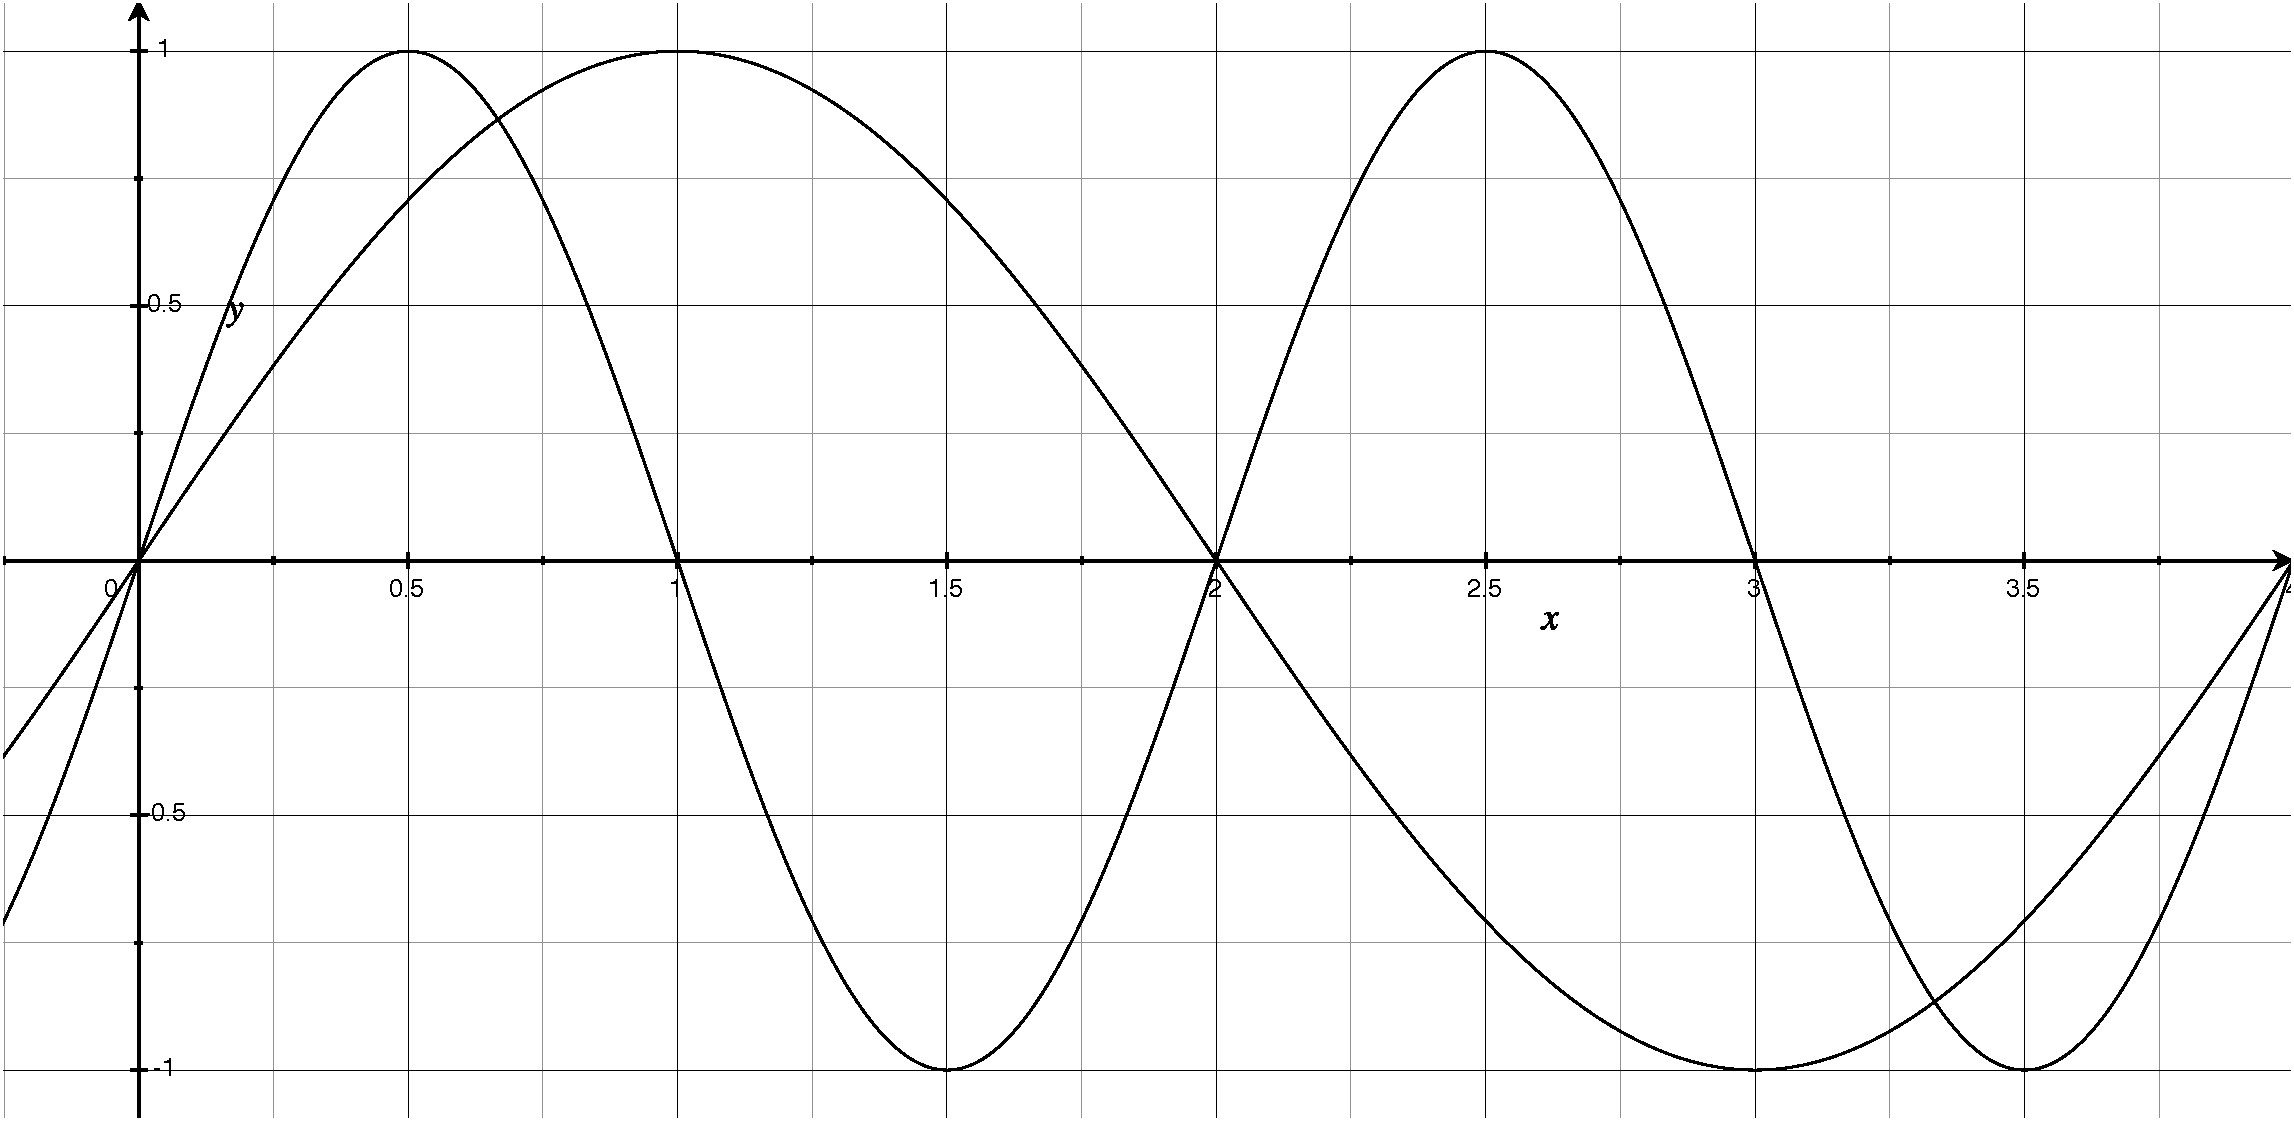
\includegraphics[width=0.6\textwidth]{sinSpeedUp.pdf}
    \caption{Graph of $\sin(\pi x/2)$ and it's ``sped up" or ``shrunken" counterpart $\sin(\pi x/2)$}
    \label{fig:sinSpedUp}
\end{figure}

Since $f(cx)$ reaches elements in its range earlier (and ``faster") than its stretched counterpart $f(x)$, the range of $f(x)$ over an interval $[x_k,x_{k+1}]$ is equivalent to the range of $f(cx)$ over the earlier and smaller interval $\left[\frac{x_k}{c},\frac{x_{k+1}}{c}\right]$. So equation \ref{eq:upperSumStretched} is equivalent to

\begin{eqnarray}
\label{eq:upperSumShrunk}
&& \frac{1}{c} \inf_{\cal{P}} \sum_{k} \sup_{\left[\frac{x_k}{c},\frac{x_{k+1}}{c}\right]} f(cx)\, l([x_k,x_{k+1}]) \nonumber \\
&=& \inf_{\cal{P}} \sum_{k} \sup_{\left[\frac{x_k}{c},\frac{x_{k+1}}{c}\right]} f(cx)\, l\left(\left[\frac{x_k}{c},\frac{x_{k+1}}{c}\right]\right)
\end{eqnarray}

The last equality comes from the fact that the length of $[x_k,x_{k+1}]$ is equal to the length of its shrunken counterpart multiplied by the shrink factor $c$. The shrink factor then cancelled out with the $1/c$ at the front of the expression.

Now it is clear though that equation \ref{eq:upperSumShrunk} is by definition $\bar{I}(f(cx))$. A parallel argument can be made for the lower sum and thus the equality is shown. Adding another term $d$ to the input make the function reach points in its range earlier, thus the function will be shifted to the left.

%%%%%%%%%
%%%%%%%%%
\item[8.] $f$ is continuous, which just means that if the two points \\$(x_1,s_1),(x_2,s_2) \in I \times S$ are less than a certain distance apart i.e. $d_{I \times S}((x_1,s_1),(x_2,s_2)) < \delta$ then $| f(x_1,s_1)-f(x_2,s_2) | < \omega(\delta)$. Now we need to show that $\varphi(y)$ has this same property, that is we need to show that if $d_S(s_1,s_2) < \delta$ then

\begin{eqnarray}
\label{eq:phiContinuous}
\left| \varphi(s_1) - \varphi(s_2) \right| &=& \left| \int_I f(x,s_1)\, dx - \int_I f(x,s_2)\, dx \right | < \omega(\delta)
\end{eqnarray}

Now we note that $d_{I \times S}((x,s_1),(x,s_2))=d_S(s_1,s_2)$ so if $d_S(s_1,s_2) < \delta$ then $d_{I \times S}((x,s_1),(x,s_2))< \delta$. Then from the continuity of $f$ this implies that $|f(x,s_1)-f(x,s_2)| < \omega(\delta)$, which in turn implies that

\begin{eqnarray}
&&\left| \int_I f(x,s_1)-f(x,s_2)\, dx \right | < l(I)\omega(\delta) \nonumber \\
&\Rightarrow& \left| \int_I f(x,s_1)\,dx- \int_I f(x,s_2)\, dx \right | < l(I)\omega(\delta) \nonumber \\
&\Rightarrow& \left| \varphi(s_1) - \varphi(s_2) \right| < l(I)\omega(\delta)
\end{eqnarray}

but this is exactly the property of continuity (equation \ref{eq:phiContinuous}) we wanted to show (up to a constant $l(I)$). The constant here is irrelevant because in words continuity means that the function can be as close as desired by making the inputs sufficiently close. The constant being there just means that we'd have to make the inputs a little closer to ensure the outputs are as close as we need them to be, but none the less we can ensure the outputs will be as arbitrarily close as need be.

%%%%%%%%%
%%%%%%%%%
\item[9.] Again we need to show that if  $d_S(s_1,s_2) < \delta$ then

\begin{eqnarray}
\label{eq:phi2Continuous}
&&\left| \varphi(s_1) - \varphi(s_2) \right| \nonumber\\
&=&\left| \int_{g_0(s_1)}^{g_1(s_1)} f(x,s_1)\, dx - \int_{g_0(s_2)}^{g_1(s_2)} f(x,s_2)\, dx \right |
\end{eqnarray}

Since $a \le g_0(y) < g_1(y) \le b$ these integrals are can be thought of as being evaluated over an interval that is to the right of $a$ by $\alpha_j := g_0(s_j)-a$ and smaller than $[a,b]$ by a factor of $\kappa_j :=l([g_0(s_j),g_1(s_j)])/l([a,b])$. From exercise 7 we know that we can stretch these functions and divide by the stretching factor to get an equivalent size interval. We can also translate the function the right to the left and still have an equivalent integral. By doing the latter first we see that \ref{eq:phi2Continuous} is equivalent to

\begin{eqnarray}
\left| \int_{a}^{g_1(s_1)-\alpha_1} f(x+\alpha_1,s_1)\, dx - \int_{a}^{g_1(s_2)-\alpha_2} f(x+\alpha_2,s_2)\, dx \right |
\end{eqnarray}

which by stretching is equivalent to

\begin{eqnarray}
\left| \frac{1}{\kappa_1} \int_{a}^{b} f\left(\frac{x+\alpha_1}{\kappa_1},s_1\right)\, dx - \frac{1}{\kappa_2} \int_{a}^{b} f\left(\frac{x+\alpha_2}{\kappa_2},s_2\right)\, dx \right|
\end{eqnarray}

and this is just the familiar condition \ref{eq:phiContinuous} from exercise 8 with a couple constant scalars that will not affect the limit.

%%%%%%%%%
%%%%%%%%%
\item[10.] This is another application of the idea from the last couple of problems: the idea that changing the input of a function makes the function reach its range faster or slower than it normally would. In this case, the ``speed" so to speak is a continuous function, so intuition would tell us that our stretch factor must also be continuous. By definition the integral is equal to its upper limit

\begin{eqnarray}
\label{eq:10start}
\int_{\varphi(a)}^{\varphi(b)} f(y)\,dy = \inf_{\cal{P}} \sum_k \sup_{[y_k,y_{k+1}]} f(y)\,l([y_k,y_{k+1}])
\end{eqnarray}

Now we must relate this quantity to a similar quantity that has its input transformed by $\varphi$. We look to an example in Figure \ref{fig:varPhiEx} for motivation.

\begin{figure}[h]
    \centering
    \includegraphics[width=0.6\textwidth]{Ch1_10.pdf}
    \caption{Example of a function $\varphi(x)$ that is differentiable and has continuous derivative on a neighborhood and positive derivative on the rest of $[a,b]$.}
    \label{fig:varPhiEx}
\end{figure}

The key point to note here is that $\varphi$ provides a continuous one-to-one map from $[x_k,x_{k+1}]$ to $[y_k,y_{k+1}]$ so the range of $f(y), y \in [y_k,y_{k+1}]$ is the exact same set as $f(\varphi(x)), x \in [x_k,x_{k+1}]$. Thus \ref{eq:10start} is equal to

\begin{eqnarray}
\label{eq:10_2}
\inf_{\cal{P}} \sum_k \sup_{[x_k,x_{k+1}]} f(\varphi(x))\,l([y_k,y_{k+1}])
\end{eqnarray}

Now note that $l([x_k,x_{k+1}]) = x_{k+1}-x_k$ and $l([y_k,y_{k+1}]) = y_{k+1}-y_k=\varphi(x_{k+1})-\varphi(x_k)$ so \ref{eq:10_2} is equal to

\begin{eqnarray}
\label{eq:10almost}
&&\inf_{\cal{P}} \sum_k \sup_{[x_k,x_{k+1}]} f(\varphi(x))\,l([y_k,y_{k+1}]) \frac{l([x_k,x_{k+1}])}{l([x_k,x_{k+1}]) } \nonumber \\
&=& \inf_{\cal{P}} \sum_k \sup_{[x_k,x_{k+1}]} f(\varphi(x))  \frac{\varphi(x_{k+1})-\varphi(x_k)}{x_{k+1}-x_k} \,l([x_k,x_{k+1}])
\end{eqnarray}

Taking smaller and smaller intervals will get \ref{eq:10almost} arbitrarily close to $\bar{I}(f(\varphi)\varphi')$ and a parallel argument can be made for the lower limit.

%%%%%%%%%
%%%%%%%%%
\item[11.] We first derive the product rule. By definition of the derivative

\begin{eqnarray}
\frac{d}{dx} (f(x) g(x)) = \lim_{h \to 0} \frac{1}{h} [f(x+h)g(x+h) - f(x)g(x)]
\end{eqnarray} 

Adding $f(x)g(x+h)-f(x)g(x+h)$ gives us

\begin{eqnarray}
&&\lim_{h \to 0} \frac{1}{h} [(f(x+h)-f(x))g(x+h) + f(x)(g(x+h)-g(x))] \nonumber \\
&=& \lim_{h \to 0} \frac{1}{h} [(f(x+h)-f(x))g(x+h)] + \lim_{h \to 0} \frac{1}{h} [f(x)(g(x+h)-g(x))] \nonumber \\
&=& f'(x)g(x) + g'(x)f(x)
\end{eqnarray} 

Thus 

\begin{equation}
\frac{d}{dx} (f(x) g(x)) = f'(x)g(x) + g'(x)f(x)
\end{equation}

And the integrals over the functions from $a$ to $b$ are also equal making the left side

\begin{equation}
[f(b)g(b)-f(a)g(a)]
\end{equation}

by the fundamental theorem of calculus and the right side equal to

\begin{equation}
\int_a^b f'(x)g(x)\, dx + \int_a^b g'(x)f(x)\,dx
\end{equation}

giving us the desired result.

%%%%%%%%%
%%%%%%%%%
\item[14.] We derive the fundamental theorem of calculus from first principles. Since $G'$ is Riemann integrable then by Corollary 1.4 when the max size of a sequence of partitions $\cal{P}$ goes to zero then

\begin{eqnarray}
\int_a^b G'(t)\,dt &=& \lim_{\nu \to \infty} \sum_{k=1}^\nu G'(\xi_{\nu k}) l(J_{\nu k})
\end{eqnarray}

where we take $\xi_{\nu k}$ to be the end point of every interval, $x_{\nu k}$. Now as $\nu \to \infty$ the end points of each interval $J_{\nu k}$ i.e. $x_{\nu k}$ and $x_{\nu k+1}$ get closer and closer so it is equivalent to write the derivative in terms of the limit of $\nu$.

\begin{eqnarray}
&&\lim_{\nu \to \infty} \sum_{k=1}^\nu \frac{G(x_{\nu x_{k+1}})-G(x_{\nu k})}{x_{\nu x_{k+1}}-x_{\nu x_{k}}} l(J_{\nu k}) \nonumber \\
&=& \lim_{\nu \to \infty} \sum_{k=1}^\nu G(x_{\nu x_{k+1}})-G(x_{\nu k}) \nonumber \\
&=& \lim_{\nu \to \infty} G(b) - G(a) \nonumber \\
&=& G(b) - G(a)
\end{eqnarray}

\end{enumerate}
%%%%%%%%%%%%%%%%
%%%%%%%%%%%%%%%%
\chapter{Lebesgue Measure on the Line}
%%%%%%%%%%%%%%%%
%%%%%%%%%%%%%%%%

There are many collections of open sets that can cover an interval $I$, these are called the covers of $I$. The covers of $I$ are themselves a set and each element in this set has a length. Thus these lengths can also be thought of a set. There is also a set of numbers that are less than or equal than all lengths in this set. The maximum of this set is the infimum of the lengths set and the outer measure of $I$.

There's always a cover of $I$ whose length is greater than the outer measure by some arbitrary length, otherwise it the outer measure wouldn't be the outer measure. 

\begin{lemma}[2.2]

\end{lemma}

\begin{proof}
We'd like to show that one can always find an open set that covers $K$ such that $m^*(\mathcal{O} \setminus K) \le \varepsilon$. We already know we can always find an open set that covers $K$ such that $m^*(\mathcal{O}) \le m^*(K) + \varepsilon$.
\end{proof}

\section{Super and Sub-Additivity}
Subadditivity means that if $S_1$ and $S_2$ are two subsets of $I$ then

\begin{equation}
\label{eq:subadditivity}
m^*(S_1 \cup S_2) \le m^*(S_1) + m^*(S_2).
\end{equation}

In words this is saying that the infimum length of all open covers of $S_1 \cup S_2$ is smaller than the sum of the infimum lengths of open covers of $S_1$ and $S_2$. There are three collections of sets in play here. There are the collections of open covers of $S_1$ and $S_2$ which we call $\{\mathcal{O}_1\}$ and $\{\mathcal{O}_2\}$ respectively and there are the collections of open covers of $S_1 \cup S_2$ which we'll call $\{\mathcal{O}_\cup\}$. Remember again these are collections of sets. There are several possible open covers. 

The key observation to make is that any if you pick any single cover from the collection $\{\mathcal{O}_1\}$, call it simply $\mathcal{O}_1$ and any cover from the collection $\{\mathcal{O}_2\}$, called $\mathcal{O}_2$ then their union $\mathcal{O}_1 \cup \mathcal{O}_2$ is also a cover of $S_1 \cup S_2$ and hence a member of the collection of open covers $\{\mathcal{O}_\cup\}$. So $\{\mathcal{O}_\cup\}$ contains all open covers of the form $\mathcal{O}_1 \cup \mathcal{O}_2$ and then some! $\{\mathcal{O}_\cup\}$ could also include covers that have smaller length than those of the form $\mathcal{O}_1 \cup \mathcal{O}_2$, which is the intuition behind the inequality \ref{eq:subadditivity}.

A similar logic can be used for inner-measures. Inner measures are defined as 

\begin{equation}
\label{eq:innerMeasure}
m_*(S) = m^*(I) - m^*(I \setminus S) = l(I) - m^*(I \setminus S)
\end{equation}

By definition we have that

\begin{eqnarray}
m_*(S_1) + m_*(S_2) = l(I)-m^*(I \setminus S_1) + l(I)-m^*(I \setminus S_2)
\end{eqnarray}

Now we are concerned with the collection of open covers of $I \setminus S_1$ and $I \setminus S_2$ respectively. Observe that the collection of open covers of $I \setminus (S_1 \cup S_2)$ is a subset of the collection of open covers that are the unions of open covers of $I \setminus S_1$ and $I \setminus S_2$.

\section*{Solutions}
\begin{enumerate}
%%%%%%%%%
%%%%%%%%%
\item[2.] Each of the $S_j$ are measurable so the difference of two consecutive $S_j$ when $j \ge 2$, i.e. $T_j :=S_j \setminus S_{j-1}$ is measurable. Now if we define $T_1 := S_1$ then 

\begin{eqnarray}
m(S_j) = m \left( \bigcup_{l = 1}^j T_j \right) = \sum_{l=1}^j m(T_j)
\end{eqnarray}

Since a measure is always greater than or equal to zero then this sum is increasing as $j$ increases, and we can always find a $j$ such that the sum is within $\epsilon > 0$ of the infinite sum $\sum_{l \ge 1} m(T_j)$ hence we write

\begin{eqnarray}
\sum_{l=1}^j m(T_j) \nearrow \sum_{l \ge 1} m(T_j)
\end{eqnarray}

But again the $T_j$ are disjoint so we have

\begin{eqnarray}
\sum_{l \ge 1} m(T_j) = m\left( \bigcup_{l \ge 1} T_j \right)  = m(S)
\end{eqnarray}

%%%%%%%%%
%%%%%%%%%
\item[3.] Since each of the $S_j$ are measurable the intersection of a finite number of them is measurable. Furthermore, the measure of the complement of a measurable set is the length of the interval minus the measure of the set so putting these together we have

\begin{eqnarray}
\label{eq:measDec}
m(S_j) = m \left( \bigcap_{l=1}^j S_j \right) = m \left( I \setminus \left[ \bigcup_{l=1}^j (I \setminus S_j) \right] \right) = l(I)- m \left(  \bigcup_{l=1}^j (I \setminus S_j)  \right)
\end{eqnarray}

We now rewrite this union as the union of disjoint sets by defining $R_1 := I \setminus S_1$

\begin{equation}
\label{eq:Rdef}
R_j := (I \setminus S_j) \setminus \left[ \bigcup_{l=1}^{j-1} (I \setminus S_l) \right]
\end{equation}

In words, each $R_j$ includes only the new elements $I \setminus S_j$ added to $\bigcup_{l=1}^{j-1} (I \setminus S_l)$ that the former didn't already have. thus we can rewrite \ref{eq:measDec} as

\begin{equation}
l(I) - m\left( \bigcup_{l=1}^j R_l \right)
\end{equation}

or since the $R_l$ are all disjoint

\begin{equation}
l(I) - \sum_{l=1}^j m\left(  R_l \right)
\end{equation}

Since measure are always greater than or equal to zero, this value decreases as $j$ increases because we're always subtracting from $l(I)$ an additional number, but it doesn't go below zero. This is because $\bigcup_{l \ge 1} R_l = S \subset I$. In fact 

\begin{equation}
\sum_{l=1}^j m\left(  R_l \right) \nearrow \sum_{l \ge1} m\left(  R_l \right) = m \left(\bigcup_{l \ge 1} R_l \right) = m \left(\bigcup_{l \ge 1} (I \setminus S_l) \right)
\end{equation}

%%%%%%%%%
%%%%%%%%%
\item[4.]  We are no longer dealing with an interval but the countable union of intervals that intersect at most one point and make up the real line i.e. $\bigcup_k I_k$. On the real line the measure of a set $S$ is define as the sum of measures of $S$ intersected with each of the intervals $I_k$ that make up $\mathbb{R}$, that is $m(S)=\sum_k m(S \cap I_k)$. The same logic for exercise 2 works for the countable union case since we did not say anything about the measure of the whole metric space. As far the countable intersection case since we still have that $S_j = \bigcap_{l=1}^j S_l$ so every time we intersect $\bigcap_{l=1}^{j-1}$ with $S_j$ we can think of the resulting set as $\bigcap_{l=1}^{j-1}$, as the running intersection with some elements taken away. Another perspective is that we are keeping a running union of the complement $\bigcup_{l=1}^{j-1} (\mathbb{R} \setminus S_l)$ and we are adding a bit each time we union it with $\mathbb{R} \setminus S_j$ to get the resulting $\bigcup_{l=1}^{j} (\mathbb{R} \setminus S_l)=\mathbb{R} \setminus S_j$. Now define $R_1 := \mathbb{R} \setminus S_1$ and define

\begin{equation}
R_j := (\mathbb{R} \setminus S_j) \setminus \left[ \bigcup_{l=1}^{j-1} (\mathbb{R} \setminus S_l) \right]
\end{equation}

to be this bit we are adding every time. Let us write the following

\begin{eqnarray}
m(S_j) &=& m(\mathbb{R} \setminus (\mathbb{R} \setminus S_j)) \nonumber\\
&=& m \left( \mathbb{R} \setminus \left[ \bigcup_{l=1}^{j} (\mathbb{R} \setminus S_l) \right] \right)\nonumber\\
&=& m\left(\mathbb{R} \setminus \bigcup_{l=1}^{j} R_l \right)
\end{eqnarray}

or by definition of measures on $\mathbb{R}$

\begin{eqnarray}
&=& \sum_k m\left(\left[ \mathbb{R} \setminus \bigcup_{l=1}^{j} R_l \right] \cap I_k \right) \nonumber \\
&=& \sum_k m\left( I_k \setminus \bigcup_{l=1}^{j} R_l  \right)\nonumber \\
&=& \sum_k \left\{ m( I_k)-m\left( \bigcup_{l=1}^{j} (R_l \cap I_k)  \right) \right\} \nonumber \\
&=& \sum_k \left\{ m( I_k)- \sum_{l=1}^j m(R_l \cap I_k)\right\}
\end{eqnarray}

 and since the $R_l$ are disjoint
 
\begin{eqnarray}
\label{eq:measureSj}
&=& \sum_k m(\mathbb{R}) - \sum_{l=0}^j m\left( R_l \right)
\end{eqnarray}
 
Notice that the union of the $R_j$ up to $j$ is $\bigcup_{l=1}^j (\mathbb{R} \setminus S_l)=(\mathbb{R} \setminus S_j)$, the $R_j$ are disjoint from each other, and they are all measurable. Since they are measurable their measure is

\begin{equation}
m(R_j) = \sum_k m(R_j \cap I_k)
\end{equation}

so let us rewrite equation \ref{eq:measureSj} as
 
\begin{eqnarray}
&=& \sum_k m(I_k) - \sum_{l=0}^j \sum_k m(R_l \cap I_k) \nonumber\\
&=& \sum_k m(I_k) - \sum_k \sum_{l=0}^j m(R_l \cap I_k) \nonumber\\
&=& \sum_k \left\{ m(I_k) -\sum_{l=0}^j  m(R_j \cap I_k) \right\}
\end{eqnarray}

Remember each $R_j$ was adding a few elements to our running union now we are just thinking about it as the elements it adds to each $I_k$. If $R_j$ adds elements that have finite measure then $\sum_k m(R_j \cap I_k)$ is finite and in that case we can switch the sums to get

\begin{eqnarray}
&=& \sum_k m(I_k) -\sum_k \sum_{l=0}^j  m(R_j \cap I_k)\nonumber \\
&=&  \sum_k \left\{ m(I_k) -\sum_{l=0}^j  m(R_j \cap I_k) \right\}
\end{eqnarray}



%%%%%%%%%
%%%%%%%%%
\item[5.] We want to prove that if a countable collection of sets $\{S_j\}$ are in a family $\mathfrak{F}$ that their intersection is as well i.e. that $\bigcap_{j \ge 1} S_j \in \mathfrak{F}$. Note that

\begin{eqnarray}
\bigcap_{j \ge 1} S_j &=& X \setminus \left( \bigcup_{j \ge 1} (X \setminus S_j) \right)
\end{eqnarray}

Each of $(X \setminus S_j)$ are in $\mathfrak{F}$ because they are complements of members of $\mathfrak{F}$. Thus the countable union and in turn its complement are all in $\mathfrak{F}$.

%%%%%%%%%
%%%%%%%%%
\item[6.] Define $S_{\cup} := \bigcup_{j \ge 1} S_j$ then

\begin{eqnarray}
\bigcap_{j \ge 1} S_j = S \setminus \left( \bigcup_{j \ge 1} (S \setminus S_j) \right)
\end{eqnarray}

%%%%%%%%%
%%%%%%%%%
\item[7.] For any rational number $q_1$ there is always a rational number $q_2$ we can add to it to get any third rational number $q_3$ that we desire. What about irrational numbers? Can we had a rational number to $q_1$ and get $q_3 = \pi$? No, because $\pi$ is irrational and so there's no two rational numbers we can add that equal it. If $q_1=\pi-1/2$ we could add the rational number $1/2$ to get $q=\pi$. So by adding rational numbers to $\pi$ we can reach some irrational numbers, but we can't reach rational ones. Note we can't reach all irrational numbers, e.g. there is no rational number you can add to $\pi$ to get $\sqrt{2}$. So the rational numbers, $\pi$, $\sqrt{2}$, etc. all have associated families of numbers you can reach by adding a rational number to them. These families are called orbits and there an uncountable number of them.

If we take one element from every orbit and call this set $S$. Then we can use the elements of $S$ as a basis in the sense that we can create any number in $\mathbb{R}$ by taking one of our basis numbers and adding a rational numbers. Say from the $\pi$ orbit we choose $\pi$, then we can create $3.26459...=\pi+3.23$ by simply adding $3.23$ to $\pi$.  

Now let $S_\alpha$ be $S$ all the elements of $S$ shifted by $\alpha$, so if $\pi \in S$ then $\pi+\alpha \in S_\alpha$. Now lets examine the countable union $\bigcup_{\alpha \in \mathbb{Q}} S_\alpha$. By construction this union equals the real line. On the other hand each $S_\alpha$ is disjoint from every other $S_\alpha$ also by construction but they all have the same measure.

Since $X$ has positive measure there must be some $I_k$ where $m(X \cap I_k) > 0$. Let us examine its measure

\begin{eqnarray}
0<m^*(X \cap I_k) = m^*(X \cap I_k \cap \mathbb{R}) 
\end{eqnarray}

Keep in mind since the union of all $S_\alpha$ is $\mathbb{R}$ we have

\begin{eqnarray}
= m^*(X \cap I_k \bigcup_{\alpha \in \mathbb{Q}} S_\alpha) = m^*\left(\bigcup_{\alpha \in \mathbb{Q}} (X \cap I_k \cap S_\alpha)\right)
\end{eqnarray}

By subadditivity

\begin{eqnarray}
\le \sum_{\alpha \in \mathbb{Q}}m^* (X \cap I_k \cap S_\alpha)
\end{eqnarray}

but since the $S_\alpha$ all have equal measure. Now we have that 

\begin{eqnarray}
\infty > m(I_k) \ge m_*(X \cap I_k) = m_*\left(\bigcup_{\alpha \in \mathbb{Q}} (X \cap I_k \cap S_\alpha)\right)
\end{eqnarray}

by superadditivity

\begin{eqnarray}
\ge \sum_{\alpha \in \mathbb{Q}}m_* (X \cap I_k \cap S_\alpha)
\end{eqnarray}

but all the measure of the terms in the sum are equal because the $S_\alpha$ all 

%%%%%%%%%
%%%%%%%%%
\item[8.] Figure \ref{fig:cantorSets} depicts the first few of these sets. 

\begin{figure}[h]
    \centering
    \includegraphics[width=0.8\textwidth]{cantorSets.png}
    \caption{First four Cantor Sets}
    \label{fig:cantorSets}
\end{figure}

There measure of the first few sets is $m(K_0)=1$,$m(K_1)=2/3$,$m(K_2)=4/9$. In general we have

\begin{equation}
m(K_\nu) = \left( \frac{2}{3} \right)^{\nu}
\end{equation}

From exercise 3, we know that if $K_\nu$ is a decreasing sequence of measurable subsets the measure of their limit is the limit of their measure i.e. $m(K_\nu) \searrow m(K)$ so 

\begin{equation}
m(K) = \lim_{\nu \to \infty} m(K_\nu) = \lim_{\nu \to \infty} \left( \frac{2}{3} \right)^{\nu} = 0
\end{equation}

%%%%%%%%%
%%%%%%%%%
\item[9.] Figure \ref{fig:cantorSets2} depicts the first few of these sets.

\begin{figure}[h]
    \centering
    \includegraphics[width=0.8\textwidth]{cantorSets2.png}
    \caption{First four sets $L$}
    \label{fig:cantorSets2}
\end{figure}

Each turn we are subtracting $2^{\nu-1}$ sets of size $(1/5)^\nu$

\begin{equation}
m(L) = \lim_{\nu \to \infty} m(L_\nu) = \lim_{\nu \to \infty} 1 - \sum_{n=1}^\nu 2^{n-1} \left( \frac{1}{5} \right)^{n} = \lim_{\nu \to \infty} 1 - \frac{1}{2} \sum_{n=1}^\nu \left( \frac{2}{5}^n \right)
\end{equation}

Which is equal to $1/3$.

%%%%%%%%%
%%%%%%%%%
\item[10.] In ternary, once we remove the middle third what remains is all elements of the reals from 0 to $0.1$ and all the elements from $0.2$ to 1. But note that $0.1$ is equivalent to $0.022222\cdots$. In other words, what remains after we remove the middle third is all numbers that have a ternary representation with no 1's. If we remove the middle ninth of the first interval, we get all numbers from $0$ to $0.01=0.022222\cdots$. Going on in this way we can imagine $K$ as all ternary numbers between 0 and 1 that have a representation without ones. 

If we remove the middle fifth of the unit interval we get (in quinary) all numbers between 0 and $0.2=0.1444\cdots$ and all numbers between $0.3$ and 1. So we can say that what is left is all numbers with a quinary representation that doesn't include a 2 in the first digit after the decimal. Similarly if the we remove the middle fifth from the interval $[0,0.2]_5$ we get all numbers between $0.02=0.01444\cdots$ and $0.03$. Thus the Cantor middle fifth set consists of all numbers on the unit interval that have a quinary representation with no 2's in it.

Now let us recall the set $S$ that consists of one element from each orbit of $(0,1)$ by adding rational numbers. Recall that $S$ was not measurable i.e. $m^*(S) \neq m_*(S)$. Also recall that $L$ has positive measure it includes unmeasurable portion we'll call $S_L$. Now $f(S_L)$ is a subset of $K$ therefore it's outer measure must be less than the outer measure of $K$, but the outer measure of $K$ is just zero so the outer measure of $f(S_L)$ must be zero and its greater than its inner-measure so it's inner-measure must also be zero, therefore $f(S_L)$ is a Lebesque measurable but it's pre-image is not. 

\end{enumerate}
%%%%%%%%%%%%%%%%
%%%%%%%%%%%%%%%%
\chapter{Integration on Measure Spaces}
%%%%%%%%%%%%%%%%
%%%%%%%%%%%%%%%%

A function $f(x)$ is measurable if for every open interval $J \in \mathbb{R}$ we have that $f^{-1}(J) \subset \mathfrak{F}$. Take a look at the example function $f:\mathbb{R} \to \mathbb{R}$ in Figure \ref{fig:borelFunction.}. Here let's define our measure space $\mathfrak{F}$ to be the Borel sets. 

\begin{figure}[h]
    \centering
    %\includegraphics[width=1.0\textwidth]{borelFunction.png}
    \caption{Pre-images of a decreasing sequence of open sets.}
    \label{fig:borelFunction}
\end{figure}

This function is $\mathfrak{F}$ measurable so the preimage of any open set is in $\mathfrak{F}$ i.e. it is one of the Borel sets. What about closed intervals, say for example the interval $[1.5,2]$, is the preimage of that interval in $\mathfrak{F}$? Well $(0.5,3)$ is open so its pre-image, we'll call it $(x_{a1},x_{b1}) \in \mathfrak{F}$. The interval $(1,2.5)$ is also open so its pre-image $(x_{a2},x_{b2}) \in \mathfrak{F}$. In general, the sets $(1.5-1/n,2+1/n),\, n=1,2,\cdots$ are all open so their pre-images $(x_{an},x_{bn})$ are all members of $\mathfrak{F}$.

Remember  in a measure space we always choose $\mathfrak{F}$ to be closed under countable intersections, countable unions, and complements. Thus $\bigcap_{n =1}^n(x_{an},x_{bn}) \in \mathfrak{F}$, but this intersection turns out to be the close interval $[x_a,x_b]$ which has the closed image $[1.5,2]$. So since the pre-image of the closed interval $[1.5,2]$ is indeed in $\mathfrak{F}$. 

In general, the pre-image of any borel set in $\mathbb{R}$ will always be Borel in $X$, thus we can construct it by using the open sets in $X$, which are of course pre-images of open sets in $\mathbb{R}$.

\section{Open Sets and Borel Sets}
If you have a set $S \subset \mathbb{R}$ its pre-image is the set of all $x \in X$ such that $f$ maps $x$ to an element in $S$. Now let's imagine all the subsets of $\mathbb{R}$ that have pre-images in the $\sigma$-algebra $\mathfrak{F}$, let's call this collection $\mathfrak{S}$. Let $S := \bigcup_{j \ge 1} S_j$ be the countable union of sets in $\mathfrak{S}$.  The pre-image of this set is the set of elements in $X$ that $f$ maps to it, but if an $f$ maps an element  $x \in X$ to an element  $s \in S$ it's because at least one of the constituent sets $S_j$ that make up $S$ contained that same $s$, but if that's the case the pre-image of $S_j$ will include $x$. Thus we can see that $f^{-1}(\bigcup_{j \ge 1} S_j) = \bigcup_{j \ge 1} f^{-1}(S_j) \in \mathfrak{F}$.

Similarly, for any $S \in \mathfrak{S}$ since the pre-image of $S$ is in $\mathfrak{F}$ then the complement of the pre-image $X \setminus f^{-1}(S)$ is also in $\mathfrak{F}$, but these are all the elements in $X$ that $f$ does NOT map in to $S$ which is the pre-image of $\mathbb{R} \setminus S$. 

\section{Proposition 3.2} If one of the functions $f_j$ maps an element $x$ in to the point $s \in (a,\infty]$, then $g_1$ will map $x$ to a point $s^* \ge s$ thus $s^*$ will certainly be in $(a,\infty$ and thus $x$ will be included in $g_1's$ pre-image of $(a,\infty]$.

\section{Simple Functions}
If $S_j$ are in the $\sigma$-algebra $\mathfrak{F}$ then their characteristic functions are measurable because the pre-image of any open set will be $S_j$ if the open set contains one, or it will be in $X \setminus S_j$ if the open set does not contain one. Either way, both of these are in $\mathfrak{F}$ so the pre-image of any open set is in $\mathfrak{F}$ and that's what it means for a function to be measurable. We can also define the simple functions

\begin{equation}
\label{eq:simpleFunction}
\varphi(x)=\sum_{j=1}^N a_j \chi_{S_j}(x),\; a_j \in \mathbb{R}
\end{equation}

Note that an element $x \in X$ can be in one of the $S_j$'s or some of them or none of them. It can either be in or out of each $S_j$ so there are $2^N$ possibilities for which $S_j$ a single $x$ can show up in. Thus if $x$ is just in $S_j$ then $\varphi$ will map $x$ to $a_j$. If it's in $S_j$ and $S_j$ for example then $\varphi$ will map $x$ to $a_j+a_i$. $\varphi$ will map $x$ to the sum of $a_j$'s for whatever $S_j$ it shows up in. 

These are also measurable. There are only $2^N$ points in the image at most so open sets will contain none of them, some of them or all of them. To get the pre-image of an open set just find out which of these $2^N$ points it contains. The pre-image will be union of the pre-image of all these points. It's easy to get the pre-image of one of these points. The point is the sum of some combination of the $a_j$'s e.g. $a_1+a_5+a_6$. The points that $\varphi$ will map to this value are the points $x \in X$ that show up in all three of the sets (1)$S_1,S_5,S_6$ and (2)no other sets. The point that show up in these three sets is the intersection of the three which is in $\mathfrak{F}$ since its constituents are. The points $x$ that show up in no other sets are the points that are in the compliment of the union of all the sets. This is also in $\mathfrak{F}$. Thus the points we're concerned with are the points in both of these i.e. the intersection.

Since there are only $2^N$ possibilities of values each $x$ will take on we can rewrite \ref{eq:simpleFunction} so that it is the sum of $2^N$ terms each with their own coefficient we'll call $\tilde{a}_\sigma$ and simple function of the set that $\varphi$ maps to that coefficient. We'll call that set $\tilde{S}_\sigma$. 

\section{Lemma 3.3}
\begin{lemma}
If $\varphi \in \mathfrak{G}^+(X)$, then

\begin{equation}
\lambda(A) = \int_A \varphi\, d\mu = \int \chi_A \,\varphi\, d\mu
\end{equation}

is a measure on $\mathfrak{F}$
\end{lemma}

\begin{proof}
Recall that a measure is a function $\mu: \mathfrak{F} \to [0,\infty]$ that gives the empty set measure zero, and has the countable additivity property for disjoint sets. Recall that $\varphi(x)=\sum_{j=1}^N a_j \chi_{S_j}(x)$. We can think of $\chi_A$ as a filter of $\varphi$ because it either multiples by one, effectively doing nothing, or it multiplies by zero, ``filtering out" a value of $\varphi$. The values it doesn't filter out are those that are in $A$. Thus we have

\begin{equation}
\chi_A \varphi = \sum_{j=1}^N a_j \chi_{S_j \cap A}
\end{equation}
 
and

\begin{equation}
\int \chi_A \varphi\, d\mu = \sum_{j=1}^N a_j \mu(S_j \cap A)
\end{equation}
 
This quantity is definitely greater than or equal to zero since $\varphi \in \mathfrak{G}^+$. It definitely is zero when $A$ is the empty set. Now if $A$ is the countable disjoint union $\bigcup_{j \ge 1} A_j$ then

\begin{eqnarray}
\lambda \left( \bigcup_{j \ge 1} A_j \right) &=& \sum_{j=1}^N a_j \mu \left( S_j \cap \bigcup_{j \ge 1} A_j  \right) \nonumber \\
&=& \sum_{j=1}^N a_j \mu \left( \bigcup_{j \ge 1} (S_j \cap A_j)  \right) \nonumber \\
&=& \sum_{j=1}^N a_j \sum_{j \ge 1} \mu (S_j \cap A_j) \nonumber \\
&=&  \sum_{j \ge 1} \sum_{j=1}^N a_j \mu (S_j \cap A_j) \nonumber \\
&=&  \sum_{j \ge 1} \lambda(A_j)
\end{eqnarray}
 
\end{proof}

\section{Integrals as Limits of Simple Functions}
The definition of the integral of a measurable function is

\begin{equation}
\int f\, d\mu = \sup \left\{ \int \varphi\, d\mu: 0 \le \varphi \le f,\, \varphi \in \mathfrak{G}^+ \right\}
\end{equation}

We can always find a sequence of simple functions $\varphi_j \nearrow f$. We know because one such example is the simple-2 functions $\varphi_{2j}(x)$ that takes on the closest value to $f(x)$ that is less than or equal $j$ AND also a multiple of $2^{-(j-1)}$. Figure \ref{fig:increasingSimpleFunctions} shows an example of these increasing simple functions and their integral for a particularly nice function.

\begin{figure}[h]
    \centering
    %\includegraphics[width=0.8\textwidth]{limitOfSimpleFunctions.png}
    \caption{Integral of Increasing Simple Functions.}
    \label{fig:increasingSimpleFunctions}
\end{figure}

\begin{theorem}
Given any simple function, $\varphi$, there is exists an $N$ such that for $n \ge N$

\begin{equation}
\int \varphi\, d\mu \le \int \varphi_{2n}\, d\mu
\end{equation}

and thus for a set of simple functions that include the simple-2 functions

\begin{equation}
\sup \int \varphi\, d\mu = \sup \int \varphi_{2n}\, d\mu
\end{equation}

so the integral of any measurable function can be stated as the supremum integral over all simple-2 functions
\end{theorem}

\begin{proof}
Let $0 \le \varphi \le f$ be a simple function. By definition it is of the form $\varphi = \sum_{l=1}^M a_l \chi_{S_l}$.
\end{proof}


\section{Monotone Convergence Theorem}
Remember that the measurable functions $\mathcal{M}^+$ are the set of functions from $X$ to $[0,\infty]$ such that the pre-image of any open set is a set in the $\sigma$-algebra of $X$ we are concerned with, $\mathfrak{F}$. We can have an increasing sequence of such functions which just means if you look at one slice $f_j(x)$ for a single $x$ and increase $j$ this itself is a sequence. When we say $f_j \nearrow$ then that means we have a bunch of sequences (one for each $x \in X$) that are all increasing. We know these will all converge to a measurable function $f$, and since it's measurable it'll have an integral but the Monotone Convergence Theorem says the following will hold

\begin{theorem}{Monotone Convergence}
\begin{equation}
\int f\, d\mu = \lim_{n \to \infty} \int f_n\, d\mu
\end{equation}
\end{theorem}

So let's examine $\int f_n\, d\mu$. Since $f_n$ is always greater than or equal to all functions that came before it, we know that the pre-image of every set $(a,\infty]$ is pre-image of $(a,\infty]$ with respect to $f_n$, because if an earlier function was able to map an $x$ up there then $f_n$ was able to also. One can see that this pre-image is strictly increasing as $n$ increases, thus the measure of the pre-image is $\mu(f_j^{-1}((a,\infty])) \nearrow \mu(f^{-1}(a,\infty])$.

Now in terms of simple functions less than $f_n$ and simple functions less than $n$, we know that there's a finite number of ``levels" $a_j$ that will be hit so we can think of these integrals as the levels multiplied by the measure of the $x$ that got mapped to that level, but for a given level as we just saw $f_n$ will always have mapped $x$ with a measure that's less than or equal to what $f$ has mapped. As $n$ increase however, the measures for each level will begin to get converge to the measure $f$ assigns. Thus the levels stay the same and the measures at those levels converge to the $f$ levels so the then the integrals of the simple functions match. The integrals of the measurable functions are the supremums of their respective simple functions though so we have the theorem.

\section{Fatou's Lemma}

\subsection{liminf and limsup}
Remember that for a single $x$, $f_{j}(x),\, j=1,2,\cdots$ is just a sequence of real numbers or possibly $\infty$, and a sequence is just a set with an ordering. It's clear than the infimum of a set is the infinte-set-analog to a minimum. If you imagine a sequence as a never ending line of numbers that are walking past you there are numbers that will always show up again and again. Then there are other numbers that might make a finite number of appearances and once their last appearance is made they are never to be seen again. The inf is the minimum of every number that has walked past you and every number that ever will. If you only consider the set of numbers that will always show up again and again and take the minimum of that set, then that is the liminf. 

\begin{lemma}[Fatou's]
If $f_n \in \mathcal{M}^+(X)$, then

\begin{equation}
\int (\liminf f_n)\, d\mu \le \liminf \int f_n\, d\mu
\end{equation}
\end{lemma}

\begin{proof}
For each $x \in X$ the $\liminf f_n$ will occur at some $j \in \mathbb{N} \cup \infty$. So for different $x$ this could occur at different places. The left hand side allows you to take the $\liminf$ at each $x$ make that your function then take the integral. If the gods are shining down upon us for some reason and for every $x$ the $\liminf f_n$ is reached at the same $j$ then the two sides are equal. Since this is usually not the case we have the lemma. 
\end{proof}

\section{All Measurable Functions (Not Just the Positive Ones)}
A function that takes on positive and negative values $f$ can be split in to a positive part $f^+$ that's equal to $f$ whenever $f$ is positive and 0 at all the other places, and a negative part $f^-$ that's equal to $-f$ whenever $f$ is negative and zero otherwise. Thus it's clear that $f=f^+-f^-$ and that $f^+$ and $f^-$ are both in $\mathcal{M}^+$. Also because integrals are more or less just the limit of sums of squares we can rearrange or split up how we add up the boxes

\begin{equation}
\int f\, d\mu = \int f^+\, d\mu - \int f^-\, d\mu
\end{equation}

...well almost...

\subsection{Absolute Convergence}
Sometimes we can rearrange infinite sums of areas of the boxes and sometimes we can't. There are examples of infinite sums where if you rearrange how you add everything up you'll get a different result! There is something called absolute convergence though which says that if you have a countable sum $\sum_{j \ge 1} a_j$ you can rearrange it however you want and always get the same result as long as $\sum_{j \ge 1} |a_j| < \infty$. That's not the only way you can rearrange things, but it's an easy way to check things are rearrangeable. 

Remember to get the integral of a measurable function you take get the integrals of all simple functions less than that function then you take the supremum of that set of integrals. The integrals of simple functions are just finite sums, but the supremum can turn in to an infinite sum. The statement $\int |f| d\mu < \infty$ is saying that the absolute value of this infinite sum is finite so it can be rearranged. Being able to rearrange these sums are important it gives us a semblance of consistency and predictably in a scary unpredictable world that's why we give the set of these function that have these absolutely convergent integrals the special name $\mathcal{L}^1(X,\mu)$. 

\section{$\mathcal{L}^1$}
For this set of functions $\mathcal{L}^1(X,\mu)$ the function (or mapping) $\mathfrak{J}$ is a function that maps elements of $\mathcal{L}^1(X,\mu)$ to $\mathbb{R}$. More importantly, this mapping is linear, meaning two things. The first is that

\begin{equation}
\mathfrak{J}(f_1+f_2) = \int f_1+f_2 \,d\mu = \int f_1\, d\mu + \int f_2\, d\mu
\end{equation}

That means it's equivalent to map these two functions then add up the mapping and get the mapping of the sum. This make sense though because it's just rearranging the infinite sum. The other condition is the following

\begin{equation}
\mathfrak{J}(cf) = \int cf \,d\mu = c \int f\, d\mu
\end{equation}

which again make sense because an infinite sum that is finite times a constant is the same as multiplying each term in the sum by the constant.

\section{Dominated Convergence Theorem}
\begin{theorem}
Let $f_n \in \mathcal{L}^1(X,\mu)$, for $n \in \mathbb{Z}^+$. Suppose $f: X \to \mathbb{R}$ and $f_n(x) \to f(x)$ for all $x \in X$, and suppose that there is a function $g$ satisfying

\begin{equation}
g \in \mathcal{L}^1(X,\mu),\; |f_n| \le g,\, 
\end{equation}

for all n. Then

\begin{equation}
f \in \mathcal{L}^1(X,\mu)
\end{equation}

and

\begin{equation}
\int f\, d\mu = \lim_{n \to \infty} \int f_n\, d\mu.
\end{equation}
\end{theorem}

\begin{proof}
This is sort of the like the monotone convergence theorem. $\int f\, d\mu$ and $\int f_n\, d\mu$ are both the supremum of integrals of simple functions $\varphi_j$ and $\varphi_{nj}$ which are functions that map sets in $\mathfrak{F}$ to a finite set of real numbers as we discussed before. Once you consider the supremum, the sum can be countably infinite with each term being thought of as a rectangular portion of area added. The height of this rectangle is the length of some interval, and the width is the measure of the pre-image of that interval with respect to $f$. Since $f_n$ converges to $f$ the measures will eventually match up. 

\end{proof}

\section{Egoroff's Theorem}

\subsection{Uniform Convergence}
When we say that $f_n(x) \to f(x)$ this is called point-wise convergence. It means that for any single $x$ the sequence of numbers $f_n(x)$ is convergence to $f(x)$. This just means that for any $\varepsilon >0$ we can find an $N$ such that when $n \ge N$ the difference between $f_n(x)$ and $f(x)$ is no greater than $\varepsilon$. The function is Figure \ref{fig:uniformConvergence} has this property. 

\begin{figure}[h]
    \centering
    %\includegraphics[width=0.8\textwidth]{uniformConvergence.png}
    \caption{The first 9 the continuous functions $f_n(x) := x^n$.}
    \label{fig:uniformConvergence}
\end{figure}

A stronger concept is uniform convergence. This says that for any $\varepsilon >0$ we can find an $n$ such that when $n \ge N$ then the difference between $f_n$ and $f$ is no greater than $\varepsilon$ for ANY $x$. The function $x^n$ goes to the function that is 0 on $[0,1)$ and 1 at 1. It's clear that for any $\varepsilon$ we choose if we look just look at a single $x$ then eventually $f_n(x)$ will get within $\varepsilon$ of $f(x)$ and stay there. But there will still be some $x$ that are not within $\varepsilon$. Hence the function is not uniformly convergent.

\subsection{Egoroff's Theorem}
It's clear now that we can't always guarantee uniform convergence for functions that confirm point-wise. Even though the pesky non-uniformly convergent part is always there, it gets smaller and smaller. This is more or less what Egoroff's Theorem says.

\begin{proposition}[Egoroff's Theorem]
Let $(X,\mathfrak{F}m\mu)$ be a measure space such that $\mu(X) < \infty$. Assume $f_j$ are $\mathfrak{F}$-measurable and $f_j(x) \to f(x)$ for all $x \in X$. Then, given any $\delta > 0$, there exists $B \in mathfrak{F}$ such that

\begin{equation}
\mu(B) \le \delta
\end{equation}

and $f_j \to f$ uniformly in on $X \setminus B$.
\end{proposition}

\begin{proof}
Since $f_j$ converges at least point-wise, then for any $x$ and for any $\varepsilon$ there will be a $j$ such that once you're past that $j$ then $f_j(x)$ and $f(x)$ will always agree within an amount less than $\varepsilon$. For $\varepsilon >0$ define the subset of $X$ where $f_j$ and $f$ will disagree by $\varepsilon$ or more at some point in the future (the guys that haven't caught up yet).

\begin{equation}
F_{n\varepsilon} = \{ x \in X: \exists j \ge n, |f_j(x)-f(x)| \ge \varepsilon \}.
\end{equation}

We know that $\bigcap_{n \ge 1} F_{n\varepsilon} = \emptyset$, because at some point each $x$ must fulfill it's promise to never stray more than $\varepsilon$ away, and so this implies that $\mu(F_{n\varepsilon}) \to 0$ as $n \to \infty$.

Now let's say we want to make the measure of the badly-behaved set less than $\delta$. We now know that for any $k$ we can set $\varepsilon = 2^{-k}$ and eventually we can find an $n$ such that the measure of the guys that haven't caught up is less than $2^{-k} \delta$. And notice the measure of the set $B := \bigcup_{k \ge 1} F_{n(k),2^{-k}}$ is less than $\delta$.

Now let's say on the well-behaved part we want everything to be uniformly convergent for $\varepsilon$ then pick a $k$ suck that $2^{-k} < \varepsilon$. There will be some guys liable to disagree but they are all in $B$ hence their measure is less than $\delta$. For everyone else there will be $j$ such that stay close $f(x)$

\end{proof}

\section{Relationship Between Riemann and Lebesgue Integrals}
If the set of points at which a function is discontinuous is finite then function is Riemann integrable. 

\section*{Solutions}
\begin{enumerate}

%%%%%%%%%
%%%%%%%%%
\item[5.] A measure space is complete when every possible subset of a set $A$ with measure zero is also measurable with measure zero. Let the completion of a measure space $(X,\mathfrak{F})$ that is not complete be

\begin{equation}
\bar{\mathfrak{F}} := \{ E \cup S: E \in \mathfrak{F}, S \subset F \in \mathfrak{F}, \mu(F) =0 \}
\end{equation}

The countable union of such set is $\bigcup_{j \ge 1} (E_j \cup S_j) = \left( \bigcup_{j \ge 1} E_j \right) \cup \left( \bigcup_{j \ge 1} S_j \right)$. The first countable union is in $\mathfrak{F}$ since that is a $\sigma$-algebra and the second set must be some subset of $F$ since all of its constituents are. Thus the union is of the form necessary to be in $\bar{\mathfrak{F}}$. Similarly the complement of a set $E \cup S$ is $X \setminus E \cap X \setminus S$, but notice $X \setminus S$ can be written as $X \setminus F \cup F \setminus S$. So the complement can be written in form $E \cup S$ and thus the completion is a $\sigma$-algebra. 

%%%%%%%%%
%%%%%%%%%
\item[7.] Remember again that the Lebesque integral is the supremum integral of simple functions, and the integral of simple functions is a finite sum. 

\begin{eqnarray}
\lambda(A) &=& \int \chi_A f\, d\mu \nonumber \\
&=& \sup \left\{ \int \chi_A\, \varphi\, d\mu: 0 \le \varphi \le f,\, \varphi \in \mathfrak{S}^+(X) \right\}  \nonumber \\
&=& \sup \left\{\sum_{j=1}^N a_j\, \mu(A \cap S_j): 0 \le \varphi \le f,\, \varphi \in \mathfrak{S}^+(X) \right\}  \nonumber \\
\end{eqnarray}

where $S_j$ is a subspace of $X$ that $\varphi$ assigns maps to $a_j$. If $A$ is the empty set then clearly $\mu(\emptyset \cap S_j) = \mu(\phi) = 0$, so the first requirement of a measure holds for $\lambda(A)$. The second requirement is additivity on disjoint sets, so let $A=\bigcup_j A_l$ where $A_j \in \mathfrak{F}$ and all the $A_j$ are disjoint. then $\lambda(A)$ becomes

\begin{eqnarray}
&&\sup \left\{\sum_{j=1}^N a_j\, \mu \left( \left(\bigcup_l A_l \right) \cap S_j \right): 0 \le \varphi \le f,\, \varphi \in \mathfrak{S}^+(X) \right\} \nonumber \\
&=& \sup \left\{\sum_{j=1}^N a_j\, \mu \left( \bigcup_l (A_l \cap S_j) \right): 0 \le \varphi \le f,\, \varphi \in \mathfrak{S}^+(X) \right\}
\end{eqnarray}

but since the $A_l$ are all disjoint

\begin{eqnarray}
&=& \sup \left\{\sum_{j=1}^N a_j\, \sum_l \mu (A_l \cap S_j): 0 \le \varphi \le f,\, \varphi \in \mathfrak{S}^+(X) \right\}\nonumber
\end{eqnarray}

The inside sum is either convergent to a finite number or it goes to infinity. If the former holds then it's absolutely convergent so we can switch the sums around, if the latter holds the whole thing will be infinite anyway so it doesn't matter that we switch the sums around thus

\begin{eqnarray}
&=& \sup \left\{ \sum_l \sum_{j=1}^N a_j\, \mu (A_l \cap S_j): 0 \le \varphi \le f,\, \varphi \in \mathfrak{S}^+(X) \right\}\nonumber
\end{eqnarray}

Remember again that for each $l$, $\varphi$ maps $A_l \cap S_j$ to $a_j$, and for different $l$ these sets are disjoint. So having a single $\varphi$ that maps also these sets to $a_j$ is equivalent to having the sum of $\varphi_l$ that only take non-zero value on the set $A_l \cap S_j$. Thus we have

\begin{eqnarray}
&=& \sup \sum_l \left\{\sum_{j=1}^N a_j\, \mu (A_l \cap S_j): 0 \le \varphi_l \le f,\, \varphi \in \mathfrak{S}^+(X) \right\}\nonumber
\end{eqnarray}

and the supremum of the sums is just the sum of the supremums

\begin{eqnarray}
&=& \sum_l \sup  \left\{\sum_{j=1}^N a_j\, \mu (A_l \cap S_j): 0 \le \varphi_l \le f,\, \varphi \in \mathfrak{S}^+(X) \right\} \nonumber \\
&=& \sum_l \int \chi_{A_l} f\, d\mu\nonumber \\
&=& \sum_l \lambda(A_l)
\end{eqnarray}

and thus we have that $\lambda$ is indeed a measure. This is important because in general $f$ can be some sort of probability distribution and $A$ are essentially sets of outcomes, called events, that can happen. It is comforting to know that the ``probability" of an outcome that is not in the outcome space and therefore not possible happening is zero. It's also comforting to know that if you want to know the probability of a bunch of different events happening that are disjoint (i.e. if one event happens the other can't happen) then you can just add up the probabilities of each event happening on its own.

%%%%%%%%%
%%%%%%%%%
\item[8.] $f$ is in $\mathcal{L}^1(X,\mu)$ which means that $\int |f|\, d\mu < \infty$. The left side is equal to the following by the definition of the integral

\begin{eqnarray}
\sup \left\{ \sum_{j=1}^N a_j\, \mu(S_j): 0 \le \varphi \le |f|,\, \varphi \in \mathfrak{G}^+ \right\}
\end{eqnarray}

We know there exists a simple function, $\varphi_{\varepsilon/2}$ that satisfies the criteria whose integral is only less than the integral of $|f|$ by $\varepsilon/2$, otherwise the integral of $|f|$ wouldn't be what it is. Since this is a simple function it only takes on finite many values so let $\alpha$ be the maximum of these finite values. The integral of this simple function over a set $S$ whose measure is less than $\varepsilon / (2\alpha)$ is thus at most $\varepsilon / 2$, and since its integral is no less than the the integral of $|f|$ minus $\varepsilon/2$ then the integral of $|f|$ will be at most $\varepsilon$ as long as that set $S$ has measure less than $\varepsilon/ (2\alpha)$. 

%%%%%%%%%
%%%%%%%%%
\item[9.] Uniform convergence of a sequence of functions $f_n$ means that there is for sure a certain $N$, such that once your sequence has passed it (i.e. $n \ge N$), no matter what $x \in X$ you look at you can guarantee that $f_n(x)$ will be no farther away from $f(x)$ than $\varepsilon$, for any $\varepsilon > 0$.

Egoroff's Theorem says that if you have a sequence of functions $f_n$ converging point wise to a function $f$ and if you just don't consider a portion of the measure space, $X$ these functions are defined on, then $f_n$ converges uniformly to $f$ on the resulting portion you have left. Egoroff's theorem says that this will still hold even if you require the portion you discard to be arbitrarily small (but still greater than zero). 

The dominated convergence theorem says that as long as a sequence of functions is dominated by an $\mathcal{L}^1(X,\mu)$ function then

\begin{equation}
\lim_{n \to \infty} \int f_n\, d\mu = \int \lim_{n \to \infty} f_n\, d\mu
\end{equation}

so we want to make sure that if we want to integral of $f_n$ to stay close to the integral of $f$ once we've passed a certain $n$, more specifically within $\varepsilon$. So let's start splitting the integral on the left in to two integrals, one taken over a set where $f_n$ is uniformly convergent and the other taken over a set where it's not called $B$. To ensure that the integral of $f_n$ will be within $\varepsilon$ of the integral of $f$, we'll require that each these constituent integrals be within $\varepsilon/2$ of the integrals of $f$ over the same respective regions.

Let's start with the set where $f$ is uniformly convergent i.e. $X \setminus B$. Again we want to ensure that once we pass a certain $N_{X \setminus B}$ that the following will hold

\begin{equation}
\left| \int_{X \setminus B} f_n\, d\mu - \int_{X \setminus B} f\,d\mu \right| = \left| \int_{X \setminus B} f_n-f\,d\mu \right| < \varepsilon /2
\end{equation}

or by definition of the integral of a measurable function

\begin{eqnarray}
\sup \left\{ \sum_{j=1}^N a_j\, \mu(S_j \cap X \setminus B): 0 \le \varphi \le f_n-f,\, \varphi \in \mathfrak{G}^+ \right\} < \varepsilon/2
\end{eqnarray}

Since $f_n$ converges uniformly one this region, know there's always a certain point we can pick that once we pass it $f_n-f$ is no bigger than a number bigger than zero that we specify. Let's specify this number to be $\varepsilon/(2\mu(X \setminus B))$ and call the integer we have to pass $N_{X \setminus B}$ then the integral can be no bigger than $\varepsilon/2$.

Now let's ensure we can find an integer that we'll call $N_{B}$ such that once we pass it the integral of $f_n$ over $B$ will be at most $\varepsilon/2$ away from the integral of $f$ over $B$. Again we want 

\begin{equation}
\left| \int_{B} f_n\, d\mu - \int_{B} f\,d\mu \right| = \left| \int_{B} f_n-f\,d\mu \right| < \varepsilon /2
\end{equation}

but the theorem we just proves in exercise 8 says we can accomplish this by making $B$ small enough. Thus the theorem is proved. 

%%%%%%%%%
%%%%%%%%%
\item[10.] $E_{j\varepsilon}$ the set of $x$'s where $f_j$ and $f$ disagree by more than $\varepsilon$. To say that $f_j \to f$ in measure is to say that $\mu(E_{j\varepsilon})$ can remain less than any number $\delta > 0$ as long as we have passed a certain $J$, the measure of these set of $x$'s must stay lower than a certain threshold. This means that for certain $x$, $f_j(x)$ can be close to $f(x)$ but then later not so close, but there can not be a net outflow.

Notice that the $x$'s for which $f_j(x)$ doesn't converge to $f(x)$ are the $x$'s such that $\limsup |f_j(x)-f(x)| > \varepsilon$. Thus these are the $x$'s that are in $\lim_{j \to \infty} E_{j \varepsilon}$, but the measure of this set is zero and so we have almost everywhere convergence. 

%%%%%%%%%
%%%%%%%%%
\item[11.] If $f_n \to f$ in measure we can split up the integral of $f_n$ over the regions where $f_n$ converges and the region where it doesn't. Over the region where it does the regular old dominated convergence theorem holds and over the other region the integral will be zero.

%%%%%%%%%
%%%%%%%%%
\item[12.] To strengthen the neural pathways in our brains we'll once again take a look at the explicit form of the Lebesque integral in terms of simple functions.

\begin{eqnarray}
&&\int_X \frac{|f-g|}{1+|f-g|}\, d\mu \nonumber\\
&=& \sup \left\{ \sum_{j=1}^N a_j^+\, \mu(S_j^+): 0 \le \varphi \le \left( \frac{|f-g|}{1+|f-g|}\right)^+,\, \varphi \in \mathfrak{G}^+ \right\}\nonumber\\
&-& \sup \left\{ \sum_{j=1}^N a_j^-\, \mu(S_j^-): 0 \le \varphi \le \left( \frac{|f-g|}{1+|f-g|} \right)^-,\, \varphi \in \mathfrak{G}^+ \right\}\nonumber\\
\end{eqnarray}

The right hand term is the negation of the negative portion of the function, but the function will never be negative, so the greater than zero requirement readily holds so we can just write

\begin{eqnarray}
\int_X \frac{|f-g|}{1+|f-g|}\, d\mu&=& \sup \left\{ \sum_{j=1}^N a_j\, \mu(S_j): 0 \le \varphi \le \frac{|f-g|}{1+|f-g|},\, \varphi \in \mathfrak{G}^+ \right\}\nonumber\\
\end{eqnarray}

If $f$ and $g$ are in the same equivalence class, i.e. they are equal $\mu$-a.e. then any time $a_j \neq 0$ in that sum the measure will be zero, so for the same elements of $M(X,\mathfrak{F},\mu)$ the function gives the value zero.

The last requirement of the shortest path from point $a$ to point $b$ is the direct path, i.e. not going through any intermediary points so we have must have $d(f,g) \le d(f,h)+d(h,g)$ so let's take a look at the term on the right of the inequality

\begin{eqnarray}
&&\frac{|f-h|}{1+|f-h|} + \frac{|h-g|}{1+|h-g|} \nonumber\\
&=& \frac{|f-h|+2|f-h|\,|h-g|+|h-g|}{1+|f-h| + |h-g| + |f-h|\,|h-g| }
\end{eqnarray}

we have to show this is always greater than $d(f,g)$.

%%%%%%%%%
%%%%%%%%%
\item[13.] Almost everywhere convergence means that for all $x$ in a measurable subset $X_1$ such that $\mu(X \setminus X_1)=0$ the function converges point wise. Recall the set

\begin{equation}
E_{j \varepsilon} = \{ x \in X: |f_j(x)-f(x)| > \varepsilon \}
\end{equation}

i.e. the set of $x$'s where $f_j$ and $f$ disagree by more than $\varepsilon$. This can be rewritten as

\begin{eqnarray}
E_{j \varepsilon} = \{ x \in X_1: |f_j(x)-f(x)| > \varepsilon \} \cup \{ x \in X \setminus X_1: |f_j(x)-f(x)| > \varepsilon \} \nonumber\\
\end{eqnarray}

since $X_1$ and $X \setminus X_1$ are disjoint the measure can be written as

\begin{eqnarray}
\mu(E_{j \varepsilon}) &=& \mu(\{ x \in X_1: |f_j(x)-f(x)| > \varepsilon \}) \nonumber\\
&&+\mu( \{ x \in X \setminus X_1: |f_j(x)-f(x)| > \varepsilon \}) \nonumber\\
\end{eqnarray}

since the measure space is complete the second term is zero because its a subset of $X \setminus X_1$ which it self has measure zero. As for the first term we know that we can find a subsequence such that the set keeps getting elements taken away since for every $x$ and every $\varepsilon$ we can find a $J$ that once you've passed it the two will never again differ by more than $\varepsilon$, but it could be that the set is infinite to begin with. For example $f_j(x)=\sin(x) /n$ converges to zero for every $x$ so for a certain $\varepsilon$ you'll always be removing $x$'s for that set, but still the measure will always be infinite. 

%%%%%%%%%
%%%%%%%%%
\item[14.] Define $d(x,S)$ be the infimum distance of $x$ to all elements in $S$. Now let us set

\begin{equation}
f_j(x) := \frac{jd(x,I \setminus \mathcal{O})}{1+jd(x,I \setminus \mathcal{O})}
\end{equation}

Figure \ref{fig:continuousToCharacteristic} depicts this function for the open set $(0.4,0.8)$ and $j=1,2,3,10^3,10^4,10^5,10^7$.

\begin{figure}[h]
    \centering
    %\includegraphics[width=0.8\textwidth]{continuousToCharacteristic.png}
    \caption{The first 9 the continuous functions $f_n(x) := x^n$.}
    \label{fig:continuousToCharacteristic}
\end{figure}

The elements that are not in $\mathcal{O}$ will always take on value zero since they have zero distance from themselves. The elements that are in $\mathcal{O}$ always have some positive distance from $I \setminus \mathcal{O}$. Now if we're talking about $K$ closed we use the function

\begin{equation}
f_j(x) := 1- \frac{jd(x,K)}{1+jd(x,K)}
\end{equation}

If $x\in K$ then the distance will always be zero so the function will always equal 1. On the other hand if $x \notin K$ then the distance to $K$ will always be positive and the term on the right will increase with $j$ driving the whole function down to zero.

%%%%%%%%%
%%%%%%%%%
\item[15.] For every open interval $\mathcal{O}$ and every $\varepsilon > 0$ we know there is a closed interval $K_{\varepsilon}$ with the same center as $\mathcal{O}$ such that $l(K_\varepsilon) > l(\mathcal{O}) + \varepsilon$. For each $\mathcal{O}_j$ in the countable intersection let us consider the corresponding closed sets $K_{2^j}$ such that $l(K_{2^j}) > l(\mathcal{O}_j) + l(\mathcal{O}_j)/2^j$ that get progressively closer and closer in length to their open counterparts as $j$ is larger. Now define the following function

\begin{equation}
f_n(x) :=  1- \frac{d(x, \bigcap_{j=1}^\infty K_{2^{j+n}})}{d(x, \bigcap_{j=1}^\infty K_{2^{j+n}})+d(x,X \setminus \bigcap_{j=1}^\infty \mathcal{O}_j)}
\end{equation}

Now, if $x$ is not in $\bigcap_{j=1}^\infty \mathcal{O}_j$ then that means $x$ is definitely not in the closed set $\bigcap_{j=1}^\infty K_{2^{j+n}} \subset \bigcap_{j=1}^\infty \mathcal{O}_j$. Since it is not in that closed set, it has some positive distance away from that set, otherwise it would be a limit point and hence part of the closed set. So in this case  $f_n$ will always be zero.

If $x$ is in $\bigcap_{j=1}^\infty K_{2^{j+n}}$ then for each $j$, $x \in K_{2^{j+n}}$, but remember $K_{2^{j+n}}$ is the close interval with the same center as $\mathcal{O}_j$ such that $l(K_{2^{j+n}}) > l(\mathcal{O}_j) + l(\mathcal{O}_j)/2^{j+n}$, so if $x \in  K_{2^{j+n}}$ then $d(x,X \setminus  \mathcal{O}_j) > l(\mathcal{O}_j)/2^{j+n}$ so $f_n$ is always 1 in these cases.

Now the only other case is when $x$ is not in $\bigcap_{j=1}^\infty K_{2^{j+n}}$, but it IS in $\bigcap_{j=1}^\infty \mathcal{O}_j$. In those cases you want $f_n(x)$ to be 1 certainly, but it may never, no matter how big we make $n$. The measure of that set though is

\begin{eqnarray}
m\left( \bigcup_{j=1}^\infty (\mathcal{O}_k \setminus K_{2^{j+n}}) \right) &=& \sum_{j=1}^\infty m(\mathcal{O}_k \setminus K_{2^{j+n}}) \nonumber \\
&<& \sum_{j=1}^\infty l(\mathcal{O}_j)/2^{j+n} \nonumber \\
&=& \frac{1}{2^n}\sum_{j=1}^\infty l(\mathcal{O}_j)/2^{j}
\end{eqnarray}



%%%%%%%%%
%%%%%%%%%
\item[16.] If $S \subset I$ is Lebesque measurable then we can find a compact set $K_{1/n} \subset S$ such that $m(K_{1/n}) > m(S) - 1/n$ and an open set $\mathcal{O}_{1/n} \supset S$ such that $m(\mathcal{O}_{1/n}) < m(S) + 1/n$ for any $n \in \mathbb{N}$. Since $K$ and $\mathcal{O}$ are both measurable we have

\begin{eqnarray}
m(\mathcal{O}_{1/n} \setminus K_{1/n}) &=& m(\mathcal{O}_{1/n}) - m(K_{1/n}) \nonumber \\
&<& m(S)+1/n - m(S) +1/n \nonumber\\
&=& 2/n
\end{eqnarray}

Now note that $S_0 := \bigcap_{n \ge 1} K_{1/n}$ is a $F_\sigma$ set and $S_1 := \bigcup{n \ge 1} \mathcal{O}_{1/n}$ is a $G_\delta$ set and by the above equation $m(S_1 \setminus S_0)$ must be zero.

From the previous exercise, we know we can find a sequence of continuous function that converge almost everywhere to the characteristic function of the $F_\sigma$ set $S_0$ and another sequence of continuous functions that converge almost everywhere to the characteristic set of $G_\delta$ set $S_1$. Either one of these sets will converge to the characteristic function of $S$ almost everywhere. Since $S_0 \subset S \subset S_1$ we know that $S_1 \setminus S_0 = (S_1 \setminus S) \cup (S \setminus S_0)$ and since these two sets are disjoint $m(S_1 \setminus S_0) = m(S_1 \setminus S)+m(S \setminus S_0)$ and they are both equal to zero.

%%%%%%%%%
%%%%%%%%%
\item[17.] Each simple function is the linear combination of characteristic functions of measurable set and we just showed that the characteristic function of any measurable set has a continuous sequence approximation. 

%%%%%%%%%
%%%%%%%%%
\item[18.] First we show that uniform convergence implies continuity in the limit. Assume $f_n \to f$ uniformly, i.e. for any $\varepsilon$ we can find an $N$ such that once we're past that $N$, $f_n$ will be within $\varepsilon$ of $f$ for any $x \in X$ we look at. 

Now what we need for $f$ to be continuous is that for any $\varepsilon > 0$, we can guarantee $f(y)$ is within $\varepsilon$ of $f(x)$ by making sure $y$ is wishing some $\delta$ of $x$. We know we can find an $N$ so that $f_n$ is within $\varepsilon/2$ of $f$, and $f_n$ is continuous so we can find a $\delta$ to keep us within $\varepsilon/2$ of $f_n(x)$. Thus if we stay within $\delta$ of $x$ then $f_n(y)$ will be within $\varepsilon/2$ of $f_n(x)$ and $f_n(x)$ will be within $\varepsilon/2$ of $f(x)$ therefore if we stay within $\delta$ of $x$ we will be within $\varepsilon$ of $f(x)$ which is exactly our requirement that we were trying to prove.

By Egoroff's theorem, we know we can make the function converge uniformly everywhere except a subset $B$ with measure less than $\delta$. Thus $f$ is continuous on $X \setminus B$.

%%%%%%%%%
%%%%%%%%%
\item[20.] $S_f(t)$ goes to the entire set $X$ as $t$ goes to zero. Elements are then removed from the set as $t$ increases. Thus the measure of the set starts out as having the same measure as $X$ then decreases monotonically as elements are removed. If $f$ were a simple function then it would map measurable sets to a finite set of levels $a_n$, and each set $S_n \in X$ that $f$ maps to $a_n$ would have an associated measure $m(S_n)$. In this scenario $\Psi_f(t)$ is a decreasing step function. When $t$ is close to zero

\begin{eqnarray}
\Psi_f(t)=\mu(S_f(t))=m(\bigcup_{n=1}^N S_n)=\sum_{n=1}^N m(S_n)
\end{eqnarray}

and as $t$ increases and just passes an $a_n$ then the associated $m(S_n)$ would drop out of that sum. Thus (without loss of generality) $\Psi_f(t)$ takes on the finite values $\sum_{n=1}^N m(S_n), \sum_{n=1}^{N-1} m(S_n), \cdots, m(S_1)$, so it is a simple function and thus its integral is

\begin{eqnarray}
\int_0^\infty \Psi_f(t)\,dt &=& \sum_{j=0}^{N-1} \left( \sum_{n=1}^{N-j} m(S_n) \right)\, \mu \left(\Psi_f^{-1} \left( \sum_{n=1}^{N-j} m(S_n) \right) \right)
\end{eqnarray}

since $\Psi_f(t)$ ``drops" once it passes $a_n$ then the measure of the pre-image of those finite values is just $a_n-a_{n-1}$ where we let $a_0 := 0$ so we have

\begin{eqnarray}
\int_0^\infty \Psi_f(t)\,dt &=& \sum_{j=0}^{N-1} \left( \sum_{n=1}^{N-j} m(S_n) \right)\, (a_n-a_{n-1})\nonumber\\
&=& \sum_{j=0}^{N-1} \left( \sum_{n=1}^{N-j}  a_n m(S_n)- \sum_{n=1}^{N-j}  a_{n-1} m(S_n) \right)\,\nonumber\\
&=& \sum_{j=0}^{N-1}a_{N-j} m(S_{N-j})\,\nonumber\\
&=& \sum_{n=1}^{N} a_n\,\mu(S_n)\nonumber\\
&=& \int_X f\, d\mu
\end{eqnarray}

The integral of $f$ takes adds up the values the function takes on times the measure of the sets where it takes that value. This is equivalent to saying if you owe one person \$10, another person \$20, and yet another person \$50 you pay them each a 10,20, and 50 dollar bill respectively. The integral of $\Psi_f(t)$ would be the equivalent of first paying everybody \$10. Then paying the second and third person another \$10, then paying the last person \$30.

%%%%%%%%%
%%%%%%%%%
\item[21.] Recall that the homeomorphism discussed maps $L$ to $K$ and recall that $L$ has positive measure, but $K$ has measure zero. We can pick a measurable subset of $K$ that has measure zero but then has a pre-image that is a subset of $L$ with positive measure, but every subset of positive measure has a non-measurable subset. 


\end{enumerate}

%%%%%%%%%%%%%%%%
%%%%%%%%%%%%%%%%
\chapter{$L^p$ Spaces}
%%%%%%%%%%%%%%%%
%%%%%%%%%%%%%%%%

\section{$L^p$ $L^q$ Relationship}

If $f \in L^p(X,\mu)$ then 

\begin{equation}
\| f \|_{L^p} = \sup \{ \| fh \|_{L^1}: h \in L^q(X,\mu), \| h \|_{L^q}=1 \}.
\end{equation}

or more explicitly 

\begin{eqnarray}
&&\left[ \int_X |f(x)|^p \, d\mu(x) \right]^{1/p} \nonumber \\
&=& \sup \left\{ \int_X |f(x)h(x)| \, d\mu(x)  : h \in L^q(X,\mu),  \int_X |h(x)|^q \, d\mu(x) = 1  \right\}
\end{eqnarray}

This statement is essentially saying that if you take all $h \in L^q$ that are of size 1 and pick the one that approximates $f$ the best in terms of $f$ having the biggest $L^1$ projection on it that projection length will be the $L^p$ norm. The statement can be boiled in to two inequalities.

\subsection{Less Than}
\begin{eqnarray}
&&\left[ \int_X |f(x)|^p \, d\mu(x) \right]^{1/p} \nonumber \\
&\le& \sup \left\{ \int_X |f(x)h(x)| \, d\mu(x)  : h \in L^q(X,\mu),  \int_X |h(x)|^q \, d\mu(x) = 1  \right\}
\end{eqnarray}

If we let $h=|f^{p-1}|$ then

\begin{eqnarray}
\int_X |f(x)h(x)| \, d\mu(x) &=& \int_X |f(x) |f^{p-1}(x)| |\, d\mu(x)\nonumber \\
&=&\int_X |f(x)|^p \, d\mu(x)
\end{eqnarray}

Of course we'd have to divide $h$ by its $L^q$ norm to make sure it has length 1 so we get 

\begin{eqnarray}
\frac{1}{\| f^{p-1} \|_{L^q}} \int_X |f(x)|^p \, d\mu(x)
\end{eqnarray}

now the question is if this is greater than $\left[ \int_X |f(x)|^p \, d\mu(x) \right]^{1/p} $ that is

\begin{eqnarray}
&&\left[ \int_X |f(x)|^p \, d\mu(x) \right]^{1/p} \stackrel{?}{\le} \frac{1}{\| f^{p-1} \|_{L^q}} \int_X |f(x)|^p \, d\mu(x)
\end{eqnarray}

or since $1/p=1-1/q$

\begin{eqnarray}
&& \int_X |f(x)|^p \, d\mu(x)  \stackrel{?}{\le}  \frac{\left[ \int_X |f(x)|^p \, d\mu(x) \right]^{1/q}}{ \left[ \int_X |f(x)|^{(p-1)q} \, d\mu(x) \right]^{1/q} } \int_X |f(x)|^p \, d\mu(x)
\end{eqnarray}

so now the question is 

\begin{eqnarray}
&&\int_X |f(x)|^p \, d\mu(x)  \stackrel{?}{\le}   \int_X |f(x)|^{(p-1)q} \, d\mu(x)
\end{eqnarray}

but since $q=p/(p-1)$ the answer is that they're equal. So that specific $h$ that we picked i.e. $f^{p-1}$ divided by it's own $L^q$ norm has $L^q$ norm equal to one so it's one of the valid $h$'s so the supremum of all valid $h$.

\subsection{Greater Than}
We know that the lowest point the function $\varphi(t) := \frac{a^p}{p} t^p + \frac{b^q}{q} t^{-q}$ can reach is $ab$ thus $ab \le \varphi(1)=\frac{a^p}{p} + \frac{b^q}{q}$ thus

\begin{equation}
fg \le \frac{1}{p} f^p + \frac{1}{q} g^q
\end{equation}

so likewise

\begin{eqnarray}
\int |fg| d\mu(x) &\le& \int |\frac{1}{p} f^p + \frac{1}{q} g^q| d\mu(x) \nonumber\\
&=& \frac{1}{p}\|f\|_{L^p}^p + \frac{1}{q} \| g \|_{L^q}^q \nonumber\\
\end{eqnarray}

but note that this in turn is less than or equal to 

\begin{eqnarray}
\frac{t^p}{p}\|f\|_{L^p}^p + \frac{1}{qt^q} \| g \|_{L^q}^q \nonumber\\
\end{eqnarray}

and again the lowest point this can reach is $\|f\|_{L_p} \| g\|_{L_p}$ proving Holder's inequality. 

\section{Denseness of Continuous Functions in $L^p(X,\mu)$}
First off, for the continuous functions $C(X)$ to be dense in $L^p(X,\mu)$ we'd have to have that every function in $L^p(X,\mu)$ either is continuous or is the limit point of continuous functions, meaning that for any $\varepsilon >0$ we choose we can find a continuous function that has an $L^p$ difference of less than that. 

Now, the following functions are continuous for any compact set 

\begin{equation}
f_{K,n}(x) = [1+n\,d(x,K)]^{-1}
\end{equation}

and they converge down to the characteristic function of any compact set. Now if $A$ is a measurable set then then its measure is defined as it's outer and inner measure which are equal. So in that case

\begin{equation}
\mu(A) = \sup\{\mu(K): K \subset A \}
\end{equation}

So from this definition we can construct an increasing sequence of compact sets $K_1 \subset K_2 \subset \cdots$. The supremum of this sequence would be the countable union of all these $K_n$'s and the measure of $A$ is thus the measure of that union. $\chi_{K_j}$ is increasing towards $\chi_A$ as more elements are included and thus get mapped to one. So by the monotone convergence theorem

\begin{eqnarray}
\int \chi_A = \int \lim_{n \to \infty} \chi_{K_j} = \lim_{n \to \infty} \int \chi_{K_j}  
\end{eqnarray}

and this then implies that

\begin{eqnarray}
&&\int \lim_{n \to \infty} \int \chi_A - \lim_{n \to \infty} \int \chi_{K_j}  = 0 \nonumber\\
&\Rightarrow& \lim_{n \to \infty} \int \chi_A - \chi_{K_j}  = 0
\end{eqnarray}

since the integrand is only ever zero or one we can treat it as being an absolute value raised to any $p$ so then we have that the $L^p$ distance of the functions $\chi_A$ and $\chi_{K_j}$ goes to zero. Simple functions are just finite linear combinations of characteristic functions on measurable sets. So any simple function is the limit point of continuous functions. So we can always construct a continuous function to get arbitrarily close to a simple function in the $L^p$ sense and remember we can always construct increasing simple functions to get arbitrarily close to a measurable function from the bottom, this is in fact the definition of the integral. 

\section{Hilbert Space}

A Hilbert space $H$ is a linear space with an inner product $(u,v)$ such that

\begin{eqnarray}
(au_1+u_2,v) &=& a(u_1,v) + (u_2,v)\nonumber\\
(u,v) &=& \overline{(v,u)}\\
(u,u) &>& 0,\,u \neq 0\nonumber
\end{eqnarray}

\subsection{Cauchy's Inequality}
Cauchy's inequality says that when you have a norm defined as $\| u\| = \sqrt{(u,u)}$

\begin{equation}
|(u,v)| \le \|u\| \cdot \|v\|
\end{equation}

We prove this as follows start with (just using properties of the inner product and conjugation)

\begin{eqnarray}
0 &\le& (u-v,u-v)\nonumber\\
&=& (u,u-v)-(v,u-v)\nonumber\\
&=& \overline{(u-v,u)} - \overline{(u-v,v)}\nonumber\\
&=& \overline{(u,u)-(v,u)} - \overline{(u,v)-(v,u)}\nonumber\\
&=& (u,u)-\overline{(v,u)} - \overline{(u,v)}+(v,v)\nonumber\\
&=& (u,u)-[(u,v) + \overline{(u,v)}]+(v,v)\nonumber\\
\end{eqnarray}

the term in the square brackets becomes two times the real part of $(u,v)$ so we get

\begin{equation}
2\,\mathrm{Re}\,(u,v) \le \|u\|^2 + \|v\|^2 
\end{equation}

We know $(u,v)$  is equal to some complex number $ce^{i\theta}$ with magnitude $c$. Thus $(e^{-i\theta}u,v)=e^{-i\theta}(u,v)=e^{-i\theta}ce^{i\theta}=c$. If $u$ was multiplied by the complex scalar $e^{i\theta}$. Since the last equation holds for any complex function $u$ then it also holds for $e^{-i\theta}u$ in which case we have

\begin{eqnarray}
2\,\mathrm{Re}\,(e^{-i\theta}u,v) \le \|e^{-i\theta}u\|^2 + \|v\|^2 
\end{eqnarray}

but of course the real part here is the positive number $c$ so

\begin{eqnarray}
2 |(u,v)| &\le& \|e^{-i\theta}u\|^2 + \|v\|^2 \nonumber\\
&=& \|u\|^2 + \|v\|^2
\end{eqnarray}

The last part comes from the fact that

\begin{eqnarray}
\|e^{-i\theta}\| &=& (e^{-i\theta}u,e^{-i\theta}u) \nonumber\\
&=& e^{-i\theta} (u,e^{-i\theta}u)\nonumber\\
&=& e^{-i\theta} \overline{(e^{-i\theta}u,u)}\nonumber\\
&=& e^{-i\theta} \overline{e^{-i\theta}}(u,u)\nonumber\\
&=& (u,u)\nonumber\\
\end{eqnarray}

The smallest point the right hand side reaches is $\|u\| \cdot \|v\|$ proving Cauchy's inequality.

\subsection{Hilbert Space as a Banach Space}
if the norm defined by $\|u\| := \sqrt{(u,u)}$ holds all the properties of a norm that we need then are Hilbert space can also be considered a Banach space. The triangle inequality holds due to Cauchy's inequality more specifically

\begin{eqnarray}
\|u+v\|^2 &=& (u+v,u+v)\nonumber\\
&=&(u,u+v)+(v,u+v)\nonumber\\
&=& \overline{(u+v,u)}+\overline{(u+v,v)} \nonumber\\
&=& (u,u)+\overline{(v,u)}+\overline{(u,v)}+(v,v) \nonumber\\
&=& (u,u)+(u,v)+\overline{(u,v)}+(v,v)\nonumber\\
\end{eqnarray}

\subsection{Convexity in a Hilbert Space}

The parallelogram law for Hilbert spaces states

\begin{equation}
\|u+v\|^2 + \|u-v\|^2 = 2\|u\|^2 + 2\|v\|^2
\end{equation}

If you have a closed convex set in Hilbert space called $K$, then for any $x$ in the Hilbert space there will be a unique ``closest approximation"to $x$ called $z \in K$. Not the uniqueness here. More formally:

\begin{proposition}[4.7]
If $K \subset H$ is a nonempty, closed, convex set in a Hilbert space $H$ and if $x \in H$, then there is a unique $z \in K$ such that $d(x,K)=\| x-z\|$.
\end{proposition} 

\begin{proof}
The definition of distance to $K$ is

\begin{equation}
d(x,K) := \inf\{\|x-y\|: y \in K \}
\end{equation}

meaning that it's the distance that is less than or equal to the distances of every $y \in K$. So if we find a a sequence $y_n$ whose distance from $x$ gets arbitrarily close to $d(x,K)$ then the distance must be the limit of the distance of these $y_n$. It is possible that if we have such a sequence it ``hops around" between multiple separated regions of $K$ that each get arbitrarily close to $d(x,K)$. Think of a Taurus with a dot in the very center. There are multiple points in the taurus that are the closest to the center.

If we prove however that $y_n$ is Cauchy then there can not be any of this jumping around. We do exactly that. Using the parallelogram law with $u=y_m-x$ and $v=x-y_n$ we get

\begin{eqnarray}
\|y_m-y_n\|^2 &=& 2\|y_n-x\|^2+2\|y_m-x\|^2-4 \left\| x-\frac{1}{2} (y_n+y_m) \right\|^2
\end{eqnarray}

The key thing to notice is here is since $K$ is convex $\frac{1}{2} (y_n+y_m)$ is also is in $K$ and so that also must be greater than or equal to $d(x,K)$. Thus

\begin{equation}
\|y_m-y_n\|^2 \le 2\|y_n-x\|^2+2\|y_m-x\|^2 - 4d(x,K)^2
\end{equation}

and since the distance of $y_n$ from $x$ converges to $d(x,K)$ we have

\begin{equation}
\lim_{m,n\to \infty} \|y_m-y_n\|^2 \le 2d(x,K)^2+2d(x,K)^2 - 4d(x,K)^2 = 0
\end{equation}

so $y_n$ is Cauchy by definition and can therefore only converge to a single point.
\end{proof}


\subsection{Orthogonal Complements}
A special case of a closed convex subset of $H$ is the linear subspace $K$ and the linear subspace $K^\perp$ that is the orthogonal complement of $K$ meaning that $K^\perp$ consists of all elements in $H$ that have an inner product of zero with all the elements of $K$. 

If $x \in H$ and $P_K x$ is that unique point $K$ closest to $x$ then we can trivially write $x$ as the sum of that point in $K$ and another element $(x-P_K)$ that turns out to be an element in $K^\perp$ i.e.

\begin{equation}
x = P_K x + (x-P_Kx)
\end{equation}

To show this remember that by definition no other point in $K$ is closer to $x$ than $P_Kx$ so anything we add or subtract to $P_Kx$ will only result in an element of $K$ that is further from $x$. Thus the following function of $t$ is minimized when $t=0$, but if that's the case, the function's derivative is zero at $t=0$ which implies $\mathrm{Re}(x-P_Kx,v)$ is zero. 

\begin{eqnarray}
\Delta(t) &=& \|x-P_K x + tv\|^2\nonumber\\
&=& (x-P_Kx+tv,x-P_Kx+tv)\nonumber\\
&=& (x-P_Kx,x-P_Kx) + 2\,\mathrm{Re}(x-P_Kx,tv) +(tv,tv)\nonumber\\
&=& \|x-P_Kx\|^2 + 2t\,\mathrm{Re}(x-P_Kx,v) +t^2 \|v\|^2
\end{eqnarray}

This quantity must be greater than zero no matter what $t$ is. 

\subsection{Linear Functionals}
A useful property of Hilbert space is that when you have a linear map from the Hilbert space to $\mathbb{C}$ i.e. a linear functional or generalized function this function can actually be written as an inner product with some other element in $H$ that is unique. Formally

\begin{proposition}
If $H$ is a Hilbert space and $\varphi: H \to \mathbb{C}$ is a continuous linear map, there exists a unique $f \in H$ such that

\begin{equation}
\varphi(u) = (u,f),\, \forall u \in H
\end{equation}
\end{proposition}

\begin{proof}
We first consider the Kernel of $\varphi$ i.e. the elements in $H$ that $\varphi$ maps to zero. If $\varphi$ sends all elements to zero then $K=H$ and choosing $f$ to be zero works. If $\varphi$ doesn't send all elements to zero then there must be at least one element such that $\varphi(u) \neq 0$. The Kernel is closed because $\varphi$ is linear so we can decompose $u$ in to $u_1+u_2$ where $u_1 \in K$ and $u_2 \in K^\perp$ and use the linearity property of $\varphi$ to see that $0\neq \varphi(u_1+u_2)=\varphi(u_1)+\varphi(u_2)=\varphi(u_2)$. So since $u_2 \in K^\perp$ and $u_2$ can't be zero we deduce that $K^\perp \neq \{0\}$. 

Because $\varphi(u_2) \neq 0$ then we can find some complex constant $c$ to multiply $u_2$ by such that $\varphi(cu_2) = c \varphi(u_2)=1$ and $cu_2$ is still in $K^\perp$. Now let's say $y$ is in $K^\perp$, then so is $\varphi(y)cu_2$ because it's still just $u_2$ multiplied by a constant. Also notice that $y-\varphi(y)cu_2$ is also in $K^\perp$ because it's the different of two elements in $K^\perp$ so by linearity it will have an inner-product of zero with any element in $K$. But notice that $\varphi(y-\varphi(y) c u_2)=\varphi(y)- \varphi(y) \varphi(cu_2)=\varphi(y)- \varphi(y) 1 = 0$ so this different element must also be in $K$ since $\varphi$ maps it to zero. The only way an element can be in $K$ but still have an inner product of zero with the elements of $K$ is if it is the element zero it self.

Now we know that $y-\varphi(y)c u_2$ is the element zero. But remember $y$ was just any arbitrary element in $K^\perp$ and $cu_2$ was just the element $\varphi$ mapped to one. So any element in $K^\perp$ can be turned to zero but just subtracting a scalar times  the single element $cu_2$. In other words every element in $K^\perp$ can be written as a constant times $cu_2$. This then means that $K^\perp$ is only one-dimensional.
\end{proof}

So there is a a one-to-one correspondence between the space of continuous linear functionals that map $H$ to $\mathbb{C}$ and inner products. 

\subsection{Constructing an Orthonormal Basis of Hilbert Space}
If we assume that Hilbert space is separable (the will be shown in the exercises) then there is a countable subset of $H$ called $S=\{v_j,\, j \ge 1 \}$ and we can always find an element $v_n \in S$ such that for any $\varepsilon > 0$ and any element in $f \in H$ we have $\|f-v_n\| < 0$. It may be the case that the elements of $S$ are not linearly independent. We can pick a subset of $S$ called $\{w_j: j\ge1 \}$ such that each $w_j$ is linearly independent of all the $w_j$ before it and the linear span of $\{w_j\}$ if dense in $H$. When we don't have the $v_j$ we need we can just construct it with $w_j$'s. Now let $L_k := \mathrm{span}\{w_j: 1 \le j \le k\}$. We can construct an orthonormal set $\{u_j: j \ge 1\}$ by setting $u_1=w_1 / \|w_1\|$ and

\begin{equation}
u_{k+1} = \frac{w_{k+1}-P_k w_{k+1}}{\|w_{k+1}-P_k w_{k+1}\|}
\end{equation}

where $P_k$ is called the orthogonal projection of $P_k$ onto $L_k$ and defined as

\begin{equation}
P_k f := \sum_{j=1}^k (f,u_j)u_j
\end{equation}

Essentially what we are doing in this construction is splitting up $w_{k+1}$ in to the sum of a portion in $L_k$ and a portion in $L_k^\perp$ and subtracting off the former so we are left with an element orthogonal to those before it. Lastly we divide by it's length to make sure $u_{k+1}$ is of size one. 

Now note that

\begin{eqnarray}
\|f\|^2 &=& \|P_kf\|^2 + \|f-P_kf\|^2 \nonumber\\
&\ge& \|P_kf\|^2 \nonumber\\
&=& \sum_{j=1}^k |(f,u_j)|^2
\end{eqnarray}

So the latter is increasing towards $\|f\|^2$ which is a complex number with finite magnitude so there's only so much length left in the tail $f-P-k$ that can be added as $k$ increases. This is also why  $\|P_n f - P_k f\|$ must go to zero and hence why $P_k f$ is Cauchy and hence converges to an element in $H$ that we call $g$. If we look at the inner product of $f-g$ with a single $u_l$ we get

\begin{eqnarray}
(f-g,u_l) &=& (f,u_l) - (g,u_l)\nonumber\\
&=& (f,u_l) - \left(\sum_{j \ge 1} (f,u_j)u_j,u_l \right)\nonumber\\
&=& (f,u_l) - \sum_{j \ge 1} (f,u_j) (u_j,u_l)\nonumber\\
&=& (f,u_l) -  (f,u_l) (u_l,u_l)\nonumber\\
&=& (f,u_l) -  (f,u_l)\nonumber\\
&=& 0\nonumber\\
\end{eqnarray}  

So $f-g$ is orthogonal to every single $u_l$ and hence every element in the span of $u_l$. The span of $u_l$ is of course all of $H$ however, so $f-g$ has an inner product of zero with all elements of $H$ so $f-g$ must be zero. This then proves that $g$ is indeed equal to $f$.

\section{$L^2(X,\mu)$}
Since $L^2$ is a Hilbert space we know that any linear functional $\varphi(u)$ can be written as the inner product of $u$ with some unique function i.e. $(u,f) = \int u(x) \overline{f(x)}\, d\mu(x)$.

\section{Radon-Nikodyn}
Let us consider two finite measures $\mu,\nu$ on $(X,\mathfrak{F})$ and two more finite measures $\alpha := \mu + 2\nu$ and $\omega := 2\mu + \nu$. We can have a linear function $\varphi: H \to \mathbb{C}$ given by

\begin{eqnarray}
\varphi(f) &=& \int_X f(x)\, d\omega(x)\nonumber\\
\end{eqnarray}

Where in this case the $H$ is $L^2(X,\alpha)$.This map is linear. Note that for two functions $f_1$ and $f_2$ in the Hilbert space we have

\begin{eqnarray}
\varphi(f_1) - \varphi(f_2) &=& \int_X f_1-f_2\, d\omega\nonumber\\
&\le& 2 \int_X f_1-f_2\, d\alpha \nonumber\\
&\le& 2 \| f_1 - f_2 \|_{L^2(X,\alpha)}^2 \nonumber\\
\end{eqnarray}

so the function is continuous because we just have to make sure $f_1$ and $f_2$ and sufficiently close and we know $\varphi(f_1) - \varphi(f_2)$ will be sufficiently close. So since the function is linear, continuous, and bounded we know we can represent it equivalently as an inner product with some function $g \in L^2(X,\alpha)$ which then means for any $f \in L^2(X,\alpha)$

\begin{eqnarray}
&&\int_X f(x)\, d\omega(x) = \int_X f(x) g(x)\, d\alpha(x)\nonumber \nonumber\\
&\Rightarrow& \int_X f(x)\, d(2\mu+\nu)(x) = \int_X f(x) g(x)\, d(\mu+2\nu)(x)\nonumber \\
&\Rightarrow& 2\int_X f(x)\, d\mu(x) + \int_X f(x)\, d\nu(x) = \int_X f(x) g(x)\, d\mu+ 2 \int_X f(x) g(x)\, d\nu(x)\nonumber \\
&\Rightarrow& \int_X f(x) (2-g(x))\, d\mu(x) = \int_X f(x) (2g(x)-1)\, d\nu(x)
\end{eqnarray}

This tells us that for any $f$ we can get the value of the integral with respect to whichever measure we'd like we just have to normalize by some other function of $g$.

Since this identity must hold for any $f \in L^2(X,\alpha)$ then it must hold for the characteristic function of any measurable sets. In particular we can define the measurable sets $S_{1l} := \{x \in X: g(x) < 1/2-1/l \}$ and $S_{2l} := \{x \in X: g(x) > 2+ 1/l\}$. If $f$ was the characteristic function of $S_{1l}$ then the left side would be non-negative, but the right side would have to non-positive, but since the identity is true then we must conclude that the measure of those sets with respect to $\mu$ and $\nu$ are both zero. We see the same thing for $S_{2l}$. Therefore it doesn't matter what values $g$ takes on those two sets. We can just say $g$ takes value zero on those sets so that get a $g$ that between 1/2 and 2.

Furthermore, whenever $g=1/2$ (we'll call this set $Z$) the right integral will be zero so $\mu$ must have measure zero on those sets. If we assume $\nu << \mu$ i.e. $\nu$ is absolutely continuous with respect to $\mu$ i.e. whenever $\mu$ assigns a set measure zero, $\nu$ will also assign the set measure zero,  it makes sense to consider

\begin{equation}
\int_X F(x)\, d\nu(x) = \int_X F(x) h(x)\, d\mu(x)
\end{equation}

where

\begin{equation}
f(x) = \frac{F(x)}{2g(x)-1},\; h(x)=\frac{2-g(x)}{2g(x)-1}
\end{equation}

\subsection{Mutually Singular Measures}
We assumed that since $\nu << \mu$ then the fact that $h(x)$ has a zero in the denominator should not matter because $\mu$ had measure zero whenever that happened and thus so did $\nu$. What if $\mu$ has measure zero, but $\nu$ does not? We'd have

\begin{equation}
\int_{X \setminus Z} F\, d\nu = \int_{X \setminus Z} Fh\, d\nu
\end{equation}

that is to say that everything is still find except for on the sets where $g(x)=1/2$.

Now let's define the measure $\lambda(E) := \nu(X \setminus Z \cap E)$. Say that whenever $g(x)=1/2$ we just set $h(x)=0$. Then we can say

\begin{equation}
\int_X F\, d\lambda = \int_X Fh\,d\mu
\end{equation}

since we changed $h$ to just be zero whenever $g=1/2$ and $\lambda$ will assign measure zero to any set in $Z$ because it will have no intersection with $X \setminus Z$ and thus it'll be the empty set which every measure must assign zero to. Now define $\rho(E)= \nu(E \cap Z)$, a measure on the sets we have trouble with. Now we can write $\nu=\lambda + \rho$. This will work because of the countable additivity of measures. $\lambda$ and $\rho$ have disjoint support and thus are said to be mutually singular. 

The following theorem says that as long as $\mu$ and $\nu$ are finite measures we can decompose $\nu$ in to the unique measures $\lambda+\rho$ where $\lambda$ is absolutely continuous with respect to $\mu$ and $\rho$ and $\mu$ have disjoint support (they are mutually singular).

\begin{theorem}
If $\mu$ and $\nu$ are finite measures on $(X,\mathfrak{F})$, then we can write

\begin{equation}
\nu = \lambda + \rho,\; \lambda << \mu,\; \rho \perp \mu
\end{equation}

and this decomposition is unique.
\end{theorem}

\begin{proof}
The only possible set where $\mu$ has measure zero and $\nu$ may not is the set where $g=1/2$, but $\lambda$ is not supported on that set i.e. it assigns that set measure zero so $\lambda << \mu$.

Now let $\tilde{\lambda}$ and $\tilde{\rho}$ be some other measures that give these properties we want i.e. we can decompose $\nu$ in to their sum, $\tilde{\lambda}$ is absolutely continuous with respect to $\mu$ and $\tilde{\rho}$ is mutually singular with respect to $\mu$ i.e. there is no set that both measures give positive measure to. Now there must be a $\tilde{Z} \in \mathfrak{F}$ such that $\tilde{\rho}$ takes its support on such that $\mu$ takes measure zero on. Now $\mu(Z \cup \tilde{Z})=0$ so $\lambda(Z \cup \tilde{Z})=0$  and $\tilde{\lambda}(Z \cup \tilde{Z})=0$ and for any  measurable $E$ we have

\begin{equation}
\lambda(E) = \lambda(E \setminus \tilde{Z}) = \nu(E \setminus (Z \cup \tilde{Z}))
\end{equation}

\begin{equation}
\tilde{\lambda}(E) = \tilde{\lambda}(E \setminus \tilde{Z}) = \nu(E \setminus (Z \cup \tilde{Z}))
\end{equation}
\end{proof}


\section*{Solutions}
\begin{enumerate}
%%%%%%%%%
%%%%%%%%%
\item[1.] If $T_j l \to T l,\, \forall l \in L$ then for any $\varepsilon$ we can find a $J$ such that once we pass it $\|T_jl - Tl\|_W < \varepsilon$. Now since $L$ is dense in $V$ then for any $v \in V$ and any $\varepsilon$ we can find an $l \in L$ such that $\|v-l\|_V < \varepsilon$.

Now we want to show we can pass a certain $J$ and guarantee that $\|T_jv-Tv\|_W < \varepsilon$, not just for any $l \in L$ but any $v \in V$. We will start by find an $l$ such that $\|v-l \|_V < \varepsilon/3C$. Thus we have

\begin{equation}
\varepsilon/3 > C \|v-l\|_V \ge \|T_j(v-l) \|_W = \|T_jv - T_j l\|_W
\end{equation} 

Since this $l \in L$ then for it we can find a $J$ such that $\|T_jl - Tl\|_W < \varepsilon/3$. Now leveraging the triangle inequality we have

\begin{eqnarray}
\|T_j v - Tv \|_W &=& \| (T_jv-T_jl) + (T_jl-Tl) + (Tv-Tl) \|_W \nonumber \\
&=& \|T_jv-T_jl\|_W + \|T_jl-Tl\|_W + \|Tv-Tl\|_W \nonumber \\
&\le& \varepsilon/3 + \varepsilon/3 + \varepsilon/3 \nonumber \\
&=& \varepsilon
\end{eqnarray}

So we know if the linear transformations converge to a transformation on $L$ then they will also converge to the same transformation on $V$.

%%%%%%%%%
%%%%%%%%%
\item[2.] $\tau_s$ is a transformation of functions that essentially ``slides" them to the right by making it so that they reach the same values they would have $s$ units later.

%%%%%%%%%
%%%%%%%%%
\item[3.] Remember that if a set $S$ is dense in a metric space $X$ then for any $\varepsilon >0$ we pick and any element $x\in X$ we pick can always find an element $s$ of $S$ such that $\|x-s\| < \varepsilon$. Separability just means that $S$ is also countable.

The functions

\begin{equation}
\varphi_{\alpha \beta}(x) := d(x, I \setminus [\alpha, \beta])
\end{equation} 

give the distance of a set $x$ to an open set $I \setminus [\alpha,\beta]$. Thus if $x \in I \setminus [\alpha,\beta]$ or if $x$ is $\alpha$ or $\beta$ then $\varphi_{\alpha \beta}(0)$. Otherwise $\varphi_{\alpha \beta}(x)$ will be some positive number. Any finite linear combination of $\varphi_{\alpha \beta}$ where $\alpha,\beta \in \mathbb{Q} \cap I$ is continuous and therefore in $C(I)$.


\end{enumerate}

%%%%%%%%%%%%%%%%
%%%%%%%%%%%%%%%%
\chapter{The Caratheodory Construction of Measures}
%%%%%%%%%%%%%%%%
%%%%%%%%%%%%%%%%

\section*{Solutions}
\begin{enumerate}
%%%%%%%%%
%%%%%%%%%
\item[1.]

%%%%%%%%%
%%%%%%%%%
\item[2.]

\end{enumerate}

%%%%%%%%%%%%%%%%
%%%%%%%%%%%%%%%%
\chapter{Product Measures}
%%%%%%%%%%%%%%%%
%%%%%%%%%%%%%%%%

\section*{Solutions}
\begin{enumerate}
%%%%%%%%%
%%%%%%%%%
\item[1.]

\end{enumerate}

%%%%%%%%%%%%%%%%
%%%%%%%%%%%%%%%%
%%%%%%%%%%%%%%%%
%%%%%%%%%%%%%%%%
%%%%%%%%%%%%%%%%
%%%%%%%%%%%%%%%%
\appendix
%%%%%%%%%%%%%%%%
%%%%%%%%%%%%%%%%
\chapter{Metric Spaces, Topological Spaces, and Compactness}
%%%%%%%%%%%%%%%%
%%%%%%%%%%%%%%%%
A metric space is a set $X$, together with a distance function $d: X \times X \to [0,\infty)$ with the properties

\begin{eqnarray}
d(x,y) &=& 0 \iff x =y\nonumber\\
d(x,y) &=& d(y,x) \\
d(x,y) \le d(x,z) + d(y,z)
\end{eqnarray}

The rational numbers with $d := | x-y |$ satisfy these conditions as does

\begin{equation}
d(x,y) := \sqrt{(x_1-y_1)^2 + \cdots + (x_n-y_n)^2}
\end{equation}

on $\mathbb{R}^n$.

\section{Sequences and Completeness}
For a sequence $(x_\nu)$ indexed by integers, if we can guarantee for any $\varepsilon$ that once we pass a certain $\nu_0$ that $d(x_\nu,y) < \varepsilon$ then we say that the sequence $(x_\nu)$ converges to $y$ or $x_\nu \to y$. 

If we can guarantee the elements of a sequence will be within a certain distance from each other we say that the sequence is a Cauchy sequence and write $d(x_\nu,x\mu) \to 0$.

A metric space is called complete if every Cauchy sequence converges to an element in the metric space. The rational numbers are not complete because you can make a sequence of rational numbers that converge to $\pi$ which is not in the set of rational numbers. 


\section{Open and Closed Sets}
In a metric space there is a notion of a ball

\begin{equation}
B_r(p) := \{x \in X: d(x,p) < r\}
\end{equation}

surround a point. A neighborhood of a point $p$ is any set that contains a ball around $p$. A set is called open if for every point you can find a ball centered at that point that is completely contained in the set. 

A point $p$ in a set is called an accumulation or limit point of a set $X$ if for any sized ball we put around $p$ there will always be a point in $X$ that is also in the ball. another way of thinking about this is that every ball around the accumulation point $p$ will have infinitely many points in $X$.

A set is called closed if it is the complement of an open set. A more useful definition is the following which says that closed sets are the sets that contain all of their accumulation points. 

\begin{proposition}[A.1]
A subset $K \subset X$ of a metric space $X$ is closed if and only if

\begin{equation}
x_j \in K,\,x_j \to p \in X \Rightarrow p \in K
\end{equation}
\end{proposition}

\begin{proof}
If $K$ is closed then $X \setminus K$ is open. If $K$ has an accumulation point $p$ then ball centered at $p$ will always contain elements of $K$, now matter how small the ball, but that means we can never find a ball around $p$ that's completely in the open set $X \setminus K$ so $p$ can only otherwise be in $K$. 

Conversely if $K$ contains all of its accumulation points then if we ever find a point $p$ such that we can't find a ball around it that only has points in $X \setminus K$ we can be ensured that point will be in $K$. Hence $X \setminus K$ only contains points that you can put a ball around with points only in $X \setminus K$ and is thus open meaning its complement $K$ is closed.
\end{proof}

The countable union of open sets is open. The reason is because if a point is in the union then its in at least one of the constituents, and since each constituent is open it'll contain a ball around that point and hence the union will also contain that ball.

A countable intersection of closed sets is closed because if a point $q$ is in the intersection then it is in each of the constituent sets. Since each of the constituent sets are closed then every ball around that point $q$ in each constituent set will contain points of the constituent set. 

The closure of a set $S$ labeled $\overline{S}$ is the smallest closed subset of $X$ that contains $S$. We can construct it by taking the intersection of all closed sets that contain $S$.

If a point $p$ is an accumulation point of $S$ then $S$ has points are as close as we'd ever like to $p$ and these points must be in every closed set that contains $S$, thus they will be in the intersection of all closed sets that contain $S$ and hence in the closure of $S$. Conversely if a point $q$ is in the closure of $S$ then every closet set that contains $S$ contains points that could get as close as we want to $q$. But if EVERY closed set that contains $S$ has all these points then we must conclude $S$ itself has all these points. 

Lastly, the interior of a set $S$ is the largest open set contained in S or the union of all open sets contained in $S$. The complement of the interior i.e. is the infinite intersection of closed sets that contain $X \setminus S$ and hence it is the closure of $X \setminus S$. 


%%%%%%%%%%%%%%%%
%%%%%%%%%%%%%%%%
\section{Compactness}
A metric space $X$ is compact if every sequence $(x_k)$ has a subsequence that converges to a point in $X$. In other words, there is a subsequence such that for any $\varepsilon >0$, after a certain point we can guarantee the subsequence never get a distance more than $\varepsilon$ away from a point in $x$ called the sequence's limit. If a subset $S \subset X$ is infinite and has an accumulation point then we can come up with a sequence of points in $S$ that we can guarantee get closer and closer to that accumulation point.  

\subsection{Total Boundedness and Separability}
A metric space $X$ is totally bounded if we can find a finite set of balls each with the same radius $\varepsilon >0$ (where $\varepsilon$ is arbitrary) that cover $X$. It turns out that compactness implies total boundedness i.e. if every infinite subset has an accumulation point then for any $\varepsilon >0$ the set can be covered with balls of that size. The formal proposition is as follows

\begin{proposition}
If $X$ is a compact metric space, then given $\varepsilon >0$ there exists a finite set $\{x_1, \cdots, x_N\}$ such that $B_\varepsilon(x_1), \cdots, B_\varepsilon(x_N)$ covers $X$.
\end{proposition}

\begin{proof}
We'll start by picking a point $x_1 \in X$ and putting a ball around it. Then we'll pick a point in $X \setminus B_\varepsilon(x_1)$ and again put a ball around it. Then we pick a point from $X \setminus (B_\varepsilon(x_1) \cup B_\varepsilon(x_2))$ and put a ball around it. Note that if we keep picking points this way none of the points will ever have a distance to any other point less that $\varepsilon$. If we never cover $X$ then the sequence $x_1, x_2,\cdots$ is an infinite sequence that never gets closer than $\varepsilon$ to any one point, but then that means it's an infinite subset of $X$ with no accumulation point so $X$ can not be compact. So if $X$ can't be covered by a finite number of balls then it is definitely not compact. So if $X$ IS compact then it can't be the case that we couldn't cover it with finite balls, we must have been able to. 
\end{proof}

Remember separability means that there is a subset that countable but also dense in $X$ i.e. for any $\varepsilon$ we can always find an element of the subset that is within that distance from any point in $X$. Compactness guarantees that there will be a countable dense subset in $X$. If we pick radii equal to $2^{-n}$ then no matter what $n$ is we know we can cover $X$ with a finite number of balls that size. We'll call each of these covers $S_n$. Now consider $\mathcal{C} := \bigcup_{n} S_n$. If we have a point $x$ in $X$ and we consider some $\varepsilon$ then there will be an $n$ such that $2^{-n} < \varepsilon$. Then that means one of the covers $S_n$ has some point that will be within $\varepsilon$ of $x$, because every point in $X$ is within the range of one of those balls and those balls only have range $2^{-n}$. So since all the points in $S_n$ are in $\mathcal{C}$ then $\mathcal{C}$ contains that point as well and $\mathcal{C}$ is also countable because it's the countable union of finite sets.

\subsection{Compactness in $\mathbb{R^n}$}

\subsection{Continuous Functions on Compact Metric Spaces}

%%%%%%%%%%%%%%%%
%%%%%%%%%%%%%%%%
\section{Product Metric Space}





\end{document}